\chapter{期望效用}

在非合作博弈中，每个结果都会给每个参与人带来一个收益，而参与人希望最大化自己的收益，收益代表了参与人对结果的偏好。到目前为止所考虑的博弈通常有纯策略均衡；在这种情况下，偏好是针对确定性结果而言的，通常也比较直观。从第 6 章开始，我们将考虑混合策略，即主动随机化的行动。此时，我们将在如下假设下分析博弈：面对随机结果时，参与人会最大化其期望收益。本章讨论的正是这一假设的合理性。

参与人的收益通常称为效用，并可用效用函数 \(u : X \rightarrow  \mathbb{R}\) 表示，其中 \(X\) 是博弈结果的集合。假设结果 \({x}_{1},\ldots ,{x}_{n}\) 分别以概率 \({p}_{1},\ldots ,{p}_{n}\) 出现；这构成结果集合上的一个彩票。该彩票 \(P\) 的期望效用为 \(\mathbb{E}\left( {u,P}\right)  = {p}_{1}u\left( {x}_{1}\right)  + \cdots  + {p}_{n}u\left( {x}_{n}\right)\) 。期望效用函数表示参与人对彩票的偏好：如果一个彩票的期望效用更高，参与人就严格偏好该彩票；如果两个彩票的期望效用相同，参与人就认为它们无差异。

博弈论的“理性”假设之一是参与人是期望效用最大化者。这个假设似乎相当强，因为它看起来意味着参与人对于所获得的效用或收益本身是“风险中性的”。然而，正如我们将在本章中解释的，这是一种误解。收益并不等同于金钱；只要参与人对彩票的偏好满足某些一致性条件，收益就可以被理解为这种偏好的一种抽象且更一般的表示。

关于参与人在彩票之间的偏好的一致性条件，被称为冯·诺依曼和摩根斯特恩(1947)公理，或基本假设。两个主要公理是

\begin{itemize}
\item 偏好是完全的，即任何两个彩票都可以比较，并且具有传递性；

\item 在一个其他部分相同的更大的复合彩票中，如果用一个彩票替换另一个彩票，那么这两个彩票之间原有的偏好或无差异关系保持不变(独立性公理)。
\end{itemize}

冯·诺依曼和摩根斯特恩(1947)定理指出，这些公理(再加上一个更具技术性的公理)保证可以构造一个期望效用函数。

我们在本章中推导这个定理。主要思想相对直接，在第一个总结部分 5.2 中进行了解释，假设(我们稍后会放宽这个假设)存在一个最不偏好的结果 \({x}_{0}\) 和一个最偏好的结果 \({x}_{1}\) 。有了这些“参考结果”，每个其他结果 \(z\) 都被替换为 \({x}_{0}\) 和 \({x}_{1}\) 之间一个与之无差异的彩票，其中 \({x}_{1}\) 以概率 \(\alpha\) 被选中。然后 \(z\) 的效用可以定义为 \(u\left( z\right)  = \alpha\) 。通过这种“效用 = 概率”的表示，期望效用定理成立，因为概率的期望仍然是概率(见图 5.1)。

这一“基础”章节的其余部分简要介绍了决策理论，该理论研究个人或群体如何在几个给定的备选方案之间做出决策(见第 5.3 节)。我们关注面临风险决策的单个参与人，即备选方案是已知结果概率的彩票(第 5.4 节)。作为决策分析的一部分，效用函数通常被用作简化复杂决策的工具，通过从人为的简单场景中引出决策者的偏好。

只有一个可能结果的彩票意味着肯定会得到该结果。因此，任何期望效用函数 \(u\) 也通过结果 \(x\) 的值 \(u\left( x\right)\) 来表示确定性条件下的偏好。如果决策仅在具有确定结果的选项之间进行，那么该效用函数被称为序数效用函数，并且可以通过应用任何严格递增变换来改变它，而不改变偏好(第5.5节)。

对于有风险的选项之间的决策，期望效用函数是基数的，这意味着只有在施加类似于温度刻度变换的正仿射变换时，偏好才会保持不变(第5.6节)。然后，通过选择一个原点 \({x}_{0}\) 来固定“效用尺度”，使得 \(u\left( {x}_{0}\right)  = 0\) ，并选择一个单位，即一个更受偏好的结果 \({x}_{1}\) ，使得 \(u\left( {x}_{1}\right)  = 1\) ，效用函数 \(u\) 就能确定了。 \(u\) 的所有其他值则已经由参与人对简单彩票的偏好所确定，这些简单彩票只有两个结果 \(x\) 和 \(y\) ，比如说，其中 \(x\) 以概率 \(1 - \alpha\) 发生， \(y\) 以概率 \(\alpha\) 发生。我们使用符号 \(x{ \land  }_{\alpha }y\) (见(5.16)，本书特有的表示法)来表示这个简单彩票，其中 \({ \land  }_{\alpha }\) 表示一个小的“概率树”，其右分支的概率为 \(\alpha\) 。

简单彩票完全规定了效用函数的值 \(u\left( z\right)\) 是如何由概率产生的，即如果参与人对 \(z\) 和简单彩票 \(x{ \land  }_{\alpha }y\) 无差异，那么 \(u\left( z\right)  = \alpha\) ，其中 \(u\left( x\right)  = 0\) 且 \(u\left( y\right)  = 1\) 。这也意味着，一旦接受了一致性公理，参与人对彩票的偏好就可以从这些简单彩票中构建出来。通过这种方式，构建效用函数是一种有用的决策辅助工具，因为具有多个结果和相应概率的彩票是相当复杂的随机方案。在实践中，如果 \(x\) 和 \(y\) 不是像可能出现的最差和最好结果那样极端，那么从概念上讲，找到一个概率 \(\alpha\) ，使得参与人对 \(z\) 和 \(x{ \land  }_{\alpha }y\) 无差异会更容易。出于这个原因，在我们的主要定理5.4中，我们甚至不假设(如第5.2节那样)存在这样的最差和最好可能结果。那么，该定理的证明就需要根据所考虑的彩票来调整效用函数的原点和单位，这会导致一些关于正仿射变换的冗长但直接的操作。

在第5.7节中，我们解释了独立性和连续性的一致性公理，这些公理意味着存在一个期望效用函数，这将在第5.8节中进行完整证明。在第5.9节中，结果本身是实数(如金额)，此时彩票具有期望值。风险厌恶意味着确定地获得这个期望值总是优于面对这个有风险的彩票，这等价于一个凹效用函数。在最后一节5.10中，我们讨论了效用公理的“理性”(作为一个简短的“哲学”讨论，我们在本书中通常避免此类讨论)，并给出了进一步的参考文献。

\section{预备知识和学习目标}

我们需要二元关系的概念，比如序关系的概念(见定义1.2)。期望值已在(4.1)中定义。

学习本章后，你应该能够

\begin{itemize}
\item 将参与人的偏好理解为结果上彩票集合中的二元关系，以及这种偏好的期望效用表示；

\item 区分确定性决策下的序数效用函数和风险决策下的基数效用函数；

\item 理解效用函数在创建完全且传递的偏好中的作用，例如对于具有多个属性的结果的加性函数(练习~\ref{exer:5.1})；

\item 解释字典序，以及为什么它在实践(见示例(5.10))和理论(见图5.3)中都存在问题；

\item 对收益应用正仿射变换，并知道为什么它们表示对彩票的相同偏好；

\item 使用简单彩票及其符号 \(x{ \land  }_{\alpha }y\) ；

\item 阐述冯·诺依曼—摩根斯特恩一致性公理及其用途；

\item 通过概率构建期望效用函数；

\item 将风险厌恶和风险中性的概念应用于本身为数值的结果。
\end{itemize}

\section{内容梗概}

本节是本章主要定理的一种“内容提要”(后续会有更多细节):如果参与人对彩票的偏好满足某些一致性公理，那么这种偏好可以用一个期望效用函数来表示。

我们研究单个决策者(此处为简便仍称为参与人)在风险下的决策。风险意味着参与人面对的是彩票，其结果 \({x}_{1},\ldots ,{x}_{n}\) 来自集合 \(X\) ，这些结果取决于具体彩票，并以已知概率 \({p}_{1},\ldots ,{p}_{n}\) 出现。为简单起见，我们仅考虑具有有限个结果的彩票，但可能结果的集合 \(X\) 可能是无限的，例如一个实数区间。

\(X\) 上的彩票集合记为 \(\Delta \left( X\right)\) 。我们从 \(\Delta \left( X\right)\) 上的二元偏好关系 \(\precsim\) 开始，其中 \(P \precsim  Q\) 表示参与人弱偏好彩票 \(Q\) 而非彩票 \(P\) 。如果 \(P \precsim  Q\) 和 \(Q \precsim  P\) 都成立，那么记为 \(P \sim  Q\) ，表示参与人对 \(P\) 和 \(Q\) 无差异。如果 \(P \precsim  Q\) 成立但 \(Q \precsim  P\) 不成立，那么这就定义了严格偏好 \(P \prec  Q\) 。

目标是研究参与人在 \(\Delta \left( X\right)\) 上的偏好关系 \(\precsim\) 应满足的条件，以便能用一个期望效用函数来表示它。这是一个函数 \(u : X \rightarrow  \mathbb{R}\) ，使得对于 \(P,Q \in  \Delta \left( X\right)\) ，

\begin{equation}
\label{eq:5.1}
P \precsim  Q\; \Leftrightarrow  \;\mathbb{E}\left( {u,P}\right)  \leq  \mathbb{E}\left( {u,Q}\right)
\end{equation}

其中 \(\mathbb{E}\left( {u,P}\right)\) 是 \(u\) 在 \(P\) 下的期望值。因此，在决策情形(以及之后的博弈中)参与人希望最大化其期望效用。

如果存在一个效用函数，那么它会对参与人的偏好 \(\precsim\) 施加一些条件。合适的条件(称为一致性公理)将足以保证期望效用函数的存在性。

第一个公理表明 \(\precsim\) 是完备且传递的。与全序(见定义 1.2)的唯一区别在于，当 \(P \neq  Q\) 时允许 \(P \sim  Q\) 成立。

\(\Delta \left( X\right)\) 中的彩票包括确定性彩票，即它们以概率 1 选择单个结果 \(x\) ，记为 \({\mathbf{1}}_{x}\) 。因此，偏好关系 \(\precsim\) 适用于确定性结果 \(x\) 和 \(y\) ，其中 \(x \precsim  y\) 代表 \({\mathbf{1}}_{x} \precsim  {\mathbf{1}}_{y}\) ，当且仅当对于期望效用函数 \(u\) 有 \(u\left( x\right)  \leq  u\left( y\right)\) 时成立。如果对于严格递增函数 \(\phi\) ，将 \(u\left( x\right)\) 替换为 \(\phi \left( {u\left( x\right) }\right)\) ，例如 \(\phi \left( u\right)  = {e}^{u}\) ，那么对确定性结果的这种偏好得以保留。也就是说，确定性结果的效用函数是序数意义上的，即更受偏好的结果具有更高的效用函数值，而这正是关键所在。

确定性条件下决策的效用函数是序数的，而风险条件下决策的期望效用函数 \(u\) 是基数的。这意味着 \(u\) 唯一允许的变换是正仿射变换，由 \({au} + b\) 给出，其中 \(a\) 和 \(b\) 为常数且 \(a > 0\) ，例如温度刻度中的摄氏度和华氏度之间的变换。这种唯一性成立是因为期望效用函数通过彩票的期望值来评估彩票。当仅考虑只有两种结果的简单彩票时，这一点就已经适用(命题5.2)。期望效用函数的“基数”性质是指它在正仿射变换下的唯一性，而不是指对结果偏好的内在“强度”。

通过应用正仿射变换，对于任意两个结果 \({x}_{0}\) 和 \({x}_{1}\) ，使得 \({x}_{0} \prec  {x}_{1}\) ，可以选择期望效用函数 \(u\) ，使得 \(u\left( {x}_{0}\right)  = 0\) 且 \(u\left( {x}_{1}\right)  = 1\) ，这就确定了效用尺度的原点和单位。现在考虑任意结果 \(z\) ，使得 \({x}_{0} \precsim  z\) 且 \(z \precsim  {x}_{1}\) (由于 \(\precsim\) 是传递的，我们将其缩写为 \({x}_{0} \precsim  z \precsim  {x}_{1}\) )。那么 \(0 \leq  u\left( z\right)  \leq  1\) ，并且 \(u\left( z\right)\) 的精确值由概率 \(\alpha\) 给出，使得参与人在 \(z\) 和以概率 \(1 - \alpha\) 选择 \({x}_{0}\) 、以概率 \(\alpha\) 选择 \({x}_{1}\) 的简单彩票之间无差异(我们将其写为 \({x}_{0}{ \land  }_{\alpha }{x}_{1}\) ，见(5.16)，其中 \({ \land  }_{\alpha }\) 表示一个小概率树)。这是因为这个简单彩票的期望效用 \(\left( {1 - \alpha }\right) u\left( {x}_{0}\right)  + {\alpha u}\left( {x}_{1}\right)\) 为 \(\alpha\) 。

通过这种缩放 \(u\left( {x}_{0}\right)  = 0\) 和 \(u\left( {x}_{1}\right)  = 1\) ，期望效用函数的每个值 \(u\left( z\right)\) 因此仅仅是选择 \({x}_{1}\) 的概率 \(\alpha\) (否则选择 \({x}_{0}\) )，该概率使得参与人在这个彩票 \({x}_{0}{ \land  }_{\alpha }{x}_{1}\) 和确定获得 \(z\) 之间无差异。这一见解具有深远的影响。为简单起见，假设在所有结果中 \({x}_{0}\) 是最不被偏好的， \({x}_{1}\) 是最被偏好的，使得对于所有结果 \(z\) 都有 \({x}_{0} \precsim  z \precsim  {x}_{1}\) 。在 \(\left\lbrack  {0,1}\right\rbrack\) 中，将 \(u\left( z\right)\) 定义为概率 \(\alpha\) ，使得 \(z \sim  {x}_{0}{ \land  }_{\alpha }{x}_{1}\) 。那么 \(\alpha\) 是唯一的，因此 \(u\) 在正仿射变换下是唯一的。
  \begin{figure}[H]\label{fig:5.1}
    \centering
    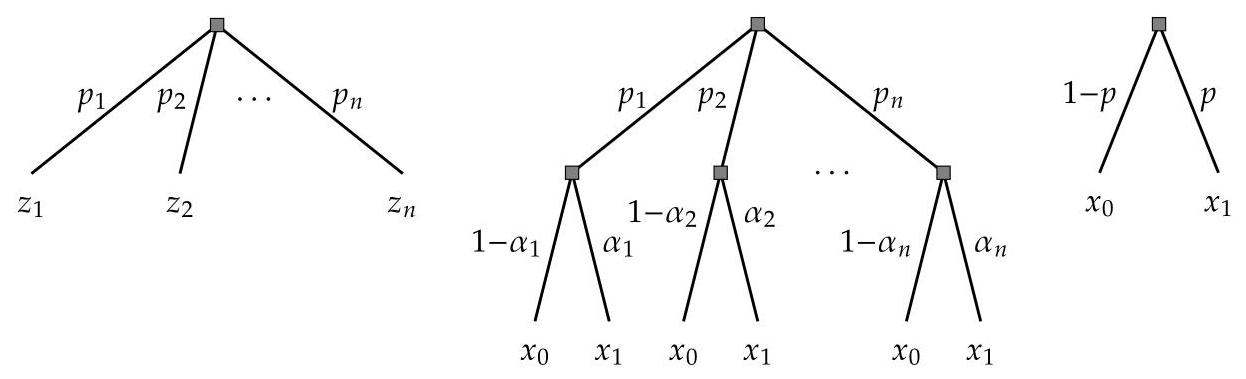
\includegraphics[width=0.8\linewidth]{images/ch05-fig01.jpg}
    \caption{彩票 \(P\) 的等价概率树，结果 \({z}_{1},\ldots ,{z}_{n}\) 的概率为 \({p}_{1},\ldots ,{p}_{n}\) ，结果 \({x}_{1}\) 的概率为 \(p = \mathop{\sum }\limits_{{i = 1}}^{n}{p}_{i}{\alpha }_{i}\) 。}
  \end{figure}
  
最重要的是，对任意彩票 \(P\) 的偏好由其期望效用 \(\mathbb{E}\left( {u,P}\right)\) 表示。即，假设 \(P\) 分别以概率 \({p}_{1},\ldots ,{p}_{n}\) 选择结果 \({z}_{1},\ldots ,{z}_{n}\) 。设 \({z}_{i} \sim  {x}_{0}{ \land  }_{{\alpha }_{i}}{x}_{1}\) ，其中对于 \(1 \leq  i \leq  n\) 有 \({\alpha }_{i} = u\left( {z}_{i}\right)\) 。图 5.1 左侧展示了 \(P\) 的概率树。在中间的树中，每个结果 \({z}_{i}\) 都被其在 \({x}_{0}\) 和 \({x}_{1}\) 之间与之无差异的简单彩票 \({x}_{0}{ \land  }_{{\alpha }_{i}}{x}_{1}\) 所替代。在该树中，唯一的结果是 \({x}_{0}\) 和 \({x}_{1}\) 。沿着从根节点出发的第 \(i\) 条边，以概率 \({p}_{i}{\alpha }_{i}\) 到达结果 \({x}_{1}\) ，因为独立概率是相乘的。对 \(i = 1,\ldots ,n\) 求和，这给出了总体概率

\begin{equation}
\label{eq:5.2}
p = \mathop{\sum }\limits_{{i = 1}}^{n}{p}_{i}{\alpha }_{i}
\end{equation}

作为 \({x}_{1}\) 的概率，而 \(1 - p\) 则是 \({x}_{0}\) 的概率。这在图 5.1 右侧的树中展示，该树汇总了 \({x}_{0}\) 和 \({x}_{1}\) 的概率。因此，参与人在 \(P\) 和 \({x}_{0}{ \land  }_{p}{x}_{1}\) 之间无差异，其中根据 (5.2) 有 \(p = \mathbb{E}\left( {u,P}\right)\) ，因为对于 \(1 \leq  i \leq  n\) 有 \({\alpha }_{i} = u\left( {z}_{i}\right)\) 。因此，不同彩票 \(P\) 和 \(Q\) 之间的比较就变成了它们对应 \({x}_{1}\) 的概率之间的比较:如果如所述有 \(p = \mathbb{E}\left( {u,P}\right)\) ，并且以类似的方式有 \(q = \mathbb{E}\left( {u,Q}\right)\) ，那么当且仅当 \(p \leq  q\) 时 \(P \precsim  Q\) ，这正是期望效用函数的性质 (5.1)。

总之，假设“参考结果” \({x}_{0}\) 和 \({x}_{1}\) ，且 \(u\left( {x}_{0}\right)  = 0\) 和 \(u\left( {x}_{1}\right)  = 1\) ，使得对于所考虑的彩票 \(P\) 的结果 \({z}_{1},\ldots ,{z}_{n}\) 有 \({x}_{0} \precsim  {z}_{i} \precsim  {x}_{1}\) 。因为效用函数的值 \(u\left( {z}_{i}\right)\) 是这些参考结果之间简单彩票 \({x}_{0}{ \land  }_{{\alpha }_{i}}{x}_{1}\) 的概率 \({\alpha }_{i}\) ，如图 5.1 所示， \(P\) 的期望效用就是如 (5.2) 中所示 \({x}_{1}\) 的汇总概率 \(p\) ，因为独立概率可以相乘。

因此，图 5.1 是期望效用函数的一种推导。关键在于，只要满足以下条件，这个论证就可以仅用偏好关系 \(\precsim\) 来进行:

\begin{itemize}
\item 如果对于结果 \({x}_{0},{x}_{1},z\) 有 \({x}_{0} \prec  z \prec  {x}_{1}\) ，那么对于某个 \(\alpha  \in  \left( {0,1}\right)\) 有 \(z \sim  {x}_{0}{ \land  }_{\alpha }{x}_{1}\) 。
\end{itemize}

\begin{itemize}
\item 如果 \(z \sim  {x}_{0}{ \land  }_{\alpha }{x}_{1}\) ，那么在任何彩票中用 \({x}_{0}{ \land  }_{\alpha }{x}_{1}\) 替换结果 \(z\) 会得到一个与之无差异的彩票。
\end{itemize}

\begin{itemize}
\item 在组合彩票中，只取决于某个结果的最终概率，而不取决于彩票的结构。
\end{itemize}

这些条件中的第一个被称为连续性公理。第二个条件，连同将 \(\sim\) 替换为 \(<\) 后的相应条件，被称为独立性公理。假定这些公理适用于一般的彩票，而不仅仅是结果。第三个条件不被视为对偏好关系的约束，因为风险决策处理的是“客观”已知的概率。

因此，彩票上任何完备、传递且满足连续性和独立性公理的偏好关系 \(\precsim\) 都可以用一个期望效用函数来表示。这就是主要的定理 5.4。其完整证明并不假定存在“极端”结果 \({x}_{0}\) 和 \({x}_{1}\) ，使得对于所有结果 \(z\) 有 \({x}_{0} \precsim  z \precsim  {x}_{1}\) ，从而通过 \(z \sim  {x}_{0}{ \land  }_{\alpha }{x}_{1}\) 来定义 \(u\left( z\right)  = \alpha\) 。相反，可以根据所考虑的彩票选择 \({x}_{0}\) 和 \({x}_{1}\) 来“局部地”定义效用函数 \(u\left( z\right)\) ，然后使用相关彩票和正仿射变换将其扩展到所有结果 \(z\) 。

本章的其余部分将更详细地解释决策理论的研究内容。对于博弈论的发展来说，除了图 5.4 中关于线段的背景材料(这在后续章节的凸性几何概念中是需要的)之外，这部分可以跳过。第 5.9 节定义了凹效用函数，这在第 11 章的讨价还价中会用到。

\section{风险决策}

以下情况说明了一个风险决策问题。假设你已经预订了一辆租车，租期为一周。你对汽车损坏的赔偿责任是 1000 欧元。在租车柜台，你可以以每天 20 欧元的成本购买额外保险，这将把你的免赔额从 1000 欧元降至零，这意味着你要额外支付 140 欧元。你应该购买这份保险吗？你的选择是：要么确定地支付 140 欧元，要么承担一个风险，即如果你损坏了汽车，就以某个概率 \(p\) 最多支付 1000 欧元。

这个决策还有一些其他的复杂情况:

\begin{itemize}
\item 这是一次性决策——你不是一直租车。如果你是，你可以自己想想，在 50 天的租车期间，你是否可能造成 1000 欧元的损坏，因为如果你一直购买这份保险，这就是你肯定要支付的金额。
\end{itemize}

\begin{itemize}
\item 如果有损坏，也许只是一个划痕，费用不到 1000 欧元。这意味着风险是由具有不同概率的多个结果定义的。
\end{itemize}

\begin{itemize}
\item 购买保险会让你安心，这样你就不必担心损坏汽车，这是额外的好处。(另一方面，你会因此开得不那么谨慎吗？)
\end{itemize}

\begin{itemize}
\item 也许租车本身只需要 200 欧元，而额外的 140 欧元会使费用大幅增加。(“独立性公理”说这应该无关紧要。)
\end{itemize}

\begin{itemize}
\item 如果你拒绝购买保险，然后不得不为损坏买单，你会后悔你的决定。在这里，决策理论家会告诉你:风险选择从定义上来说意味着你不知道未来。如果你冒了这个险，就接受你这样做的决定。
\end{itemize}

\begin{itemize}
\item 支付 1000 欧元可能会让你陷入严重的财务困境。希望不会这样。然而，这种考虑在其他情况下可能是一个很好的指导，例如你是否应该再花 80 英镑，为你新买的价值 400 英镑的冰箱购买三年的“意外故障”保险。(这种保险在英国很受欢迎，但往往定价过高。)
\end{itemize}

\begin{itemize}
\item 你不知道你的租车发生 1000 欧元损坏的概率 \(p\) 。想想在 50 天的租车使用中你是否可能造成这样的损坏，可能有助于估计这个概率。这也取决于你在访问地的驾驶安全程度。
\end{itemize}

关于概率 \(p\) ，如果你不购买保险，期望成本为 \(1,{000} \cdot  p\) 欧元；当 \(p > {0.14}\) 时，该成本超过 140 欧元。然而，并不存在“若 \(p > {0.14}\) 就购买保险”这样的规则，因为例如当 \(p = {0.1}\) 时，你也完全可能更愿意购买保险。(实际的 \(p\) 可能远低于租车公司报价所暗示的水平——单独的“租车免赔额”保险公司以每年 60 欧元的价格为多次租车承保免赔额，因此 (a) 这表明风险较低，(b) 这是一种你也许更愿意提前购买的保险。)

假设在这个租车问题中，你对自己损坏汽车的概率 \(p\) 有一个估计(为了安全起见， \(p\) 可能估计得相当高)。那么，你是否应该花 140 欧元购买额外保险的问题就被称为风险决策问题，这是决策理论中的问题之一，也是我们要研究的问题。

决策理论处理的情况在以下方面有所不同:

\begin{itemize}
\item 个人决策或群体决策；
\end{itemize}

\begin{itemize}
\item 确定性决策、风险决策或不确定性决策；
\end{itemize}

\begin{itemize}
\item 单属性结果或多属性结果。
\end{itemize}

租车问题只有一个决策者。群体决策问题是要汇总多个个体的偏好。例如，有三个候选人 \(x,y,z\) 竞争一份工作，由一个三人委员会 \(A,B,C\) 来决定，他们的偏好如下:

\[
A : x \prec  y \prec  z
\]

\begin{equation}
\label{eq:5.3}
B : \;y \prec  z \prec  x
\end{equation}

\[
C : z \prec  x \prec  y
\]

这意味着 \(A\) 对 \(y\) 的偏好高于 \(x\) ，对 \(z\) 的偏好高于 \(x\) 和 \(y\) ， \(B\) 和 \(C\) 也有相应的偏好。一种可能的决策规则是通过多数人规则进行两两比较。在这种情况下， \(A\) 和 \(B\) (多数人)对 \(z\) 的偏好高于 \(y\) ， \(A\) 和 \(C\) 对 \(y\) 的偏好高于 \(x\) ， \(B\) 和 \(C\) 对 \(x\) 的偏好高于 \(z\) 。因此，即使每个委员会成员对候选人都有严格序，但这种两两比较会产生循环，因此没有明确的获胜者。这就是孔多塞悖论，是群体决策问题之一，属于社会选择领域。在本章中，我们只考虑单个决策者及其偏好，为简洁起见，我们仍称其为参与人。

在确定性决策中，决策的结果是确定已知的。风险决策处理的情况是，结果可能是随机的，但参与人知道(必要时尽可能准确地)这些结果的概率。不确定性决策涉及的是结果的真实概率未知的情况。决策理论的一种方法(我们不讨论)是寻找关于偏好的条件，使其等价于参与人对这些结果具有某种(可能是隐含定义的)主观概率，而这些主观概率可以像普通概率一样使用。我们考虑已知概率的风险情况。

一些决策问题只涉及单一属性，如金钱，当结果确定时，通常很容易确定偏好(偏好是少支付而不是多支付)。许多决策涉及多个属性，此时决策就不再容易了，例如是去一家高档但昂贵的餐厅，还是去一家稍差但便宜的餐厅，这里涉及质量和价格两个属性。结果的属性结构对我们来说并不重要，但它有助于说明看似自然的决策规则可能出现的复杂情况，如下例 (5.10) 所示。

\section{对彩票的偏好}

我们考虑单个参与人在决策情形中的以下设定。集合 \(X\) 包含可能的结果， \(X\) 上的(有限)彩票集合 \(\Delta \left( X\right)\) 正式定义如下。

定义 5.1。设 \(X\) 是一个非空的结果集合。 \(X\) 上的一个彩票由 \(X\) 中的有限个元素 \({x}_{1},\ldots ,{x}_{n}\) (也称为 \(P\) 的结果)以及相应的概率 \({p}_{1},\ldots ,{p}_{n}\) 给出，这些概率是非负实数，且它们的和为 1。 \(X\) 上的彩票集合记为 \(\Delta \left( X\right)\) 。

如果我们比较两个彩票 \(P\) 和 \(Q\) ，我们可以假设它们对相同的结果 \({x}_{1},\ldots ,{x}_{n}\) 分配概率 \({p}_{1},\ldots ,{p}_{n}\) 和 \({q}_{1},\ldots ,{q}_{n}\) ，如有必要，若某个结果只在其中一个彩票中有正概率，则可将它在另一个彩票中的概率设为零。如果 \(X\) 本身是有限的，这是最简单的情况，此时我们可以取 \(n = \left| X\right|\) ，但我们也可以考虑 \(X\) 为无限的情况。

我们假设参与人对任意两个彩票 \(P\) 和 \(Q\) 有偏好。如果在面对 \(P\) 和 \(Q\) 之间的选择时，参与人愿意选择 \(Q\) 而不是 \(P\) ，我们将其记为

\[
P \lesssim  Q
\]

并且也说参与人(弱)偏好 \(Q\) 甚于 \(P\) 。然后我们通过以下方式定义无差异关系 \(\sim\)

\begin{equation}
\label{eq:5.4}
P \sim  Q\; \Leftrightarrow  \;P \precsim  Q\text{ and }Q \precsim  P
\end{equation}

其中 \(P \sim  Q\) 表示参与人对 \(P\) 和 \(Q\) 无差异。严格偏好关系 \(\prec\) 定义为

\begin{equation}
\label{eq:5.5}
P \prec  Q\; \Leftrightarrow  \;P \precsim  Q\text{ and }\operatorname{not}Q \precsim  P
\end{equation}

其中 \(P \prec  Q\) 表示参与人严格偏好 \(Q\) 甚于 \(P\) ；显然它等价于

\[
P \prec  Q\; \Leftrightarrow  \;P \precsim  Q\text{ and }\operatorname{not}P \sim  Q.
\]

我们将推导出 \(\Delta \left( X\right)\) 上的弱偏好关系 \(\precsim\) 的一些条件，这些条件使该关系在决策理论和博弈论中的应用在数学上易于处理。这些将是对 \(\precsim\) 的限制，它们可能无法描述人们在某些决策情况下的实际行为。相反，这些限制通常被称为规范性条件，也就是说，它们说明了人们应该如何行动，例如为了得出一个确定的决策。这样，该理论可以用作决策分析的工具。

目标是找到一个函数 \(u : X \rightarrow  \mathbb{R}\) 的存在条件。该函数称为参与人的效用函数，并使得：如果彩票 \(Q\) 的期望效用高于彩票 \(P\) 的期望效用，参与人就严格偏好彩票 \(Q\) 而非彩票 \(P\) ；如果两张彩票的期望效用相同，参与人对它们无差异。

期望效用是给定彩票的效用函数的期望值。假设彩票 \(P\) 对于结果 \({x}_{1},\ldots ,{x}_{n}\) 分别有概率 \({p}_{1},\ldots ,{p}_{n}\) 。那么应用于这些结果的效用函数 \(u\) 定义了一个随机变量。作为 (4.1) 的扩展，我们用 \(\mathbb{E}\left( {u,P}\right)\) 表示其期望值，表达式为

\begin{equation}
\label{eq:5.6}
\mathbb{E}\left( {u,P}\right)  = {p}_{1}u\left( {x}_{1}\right)  + \cdots  + {p}_{n}u\left( {x}_{n}\right) .
\end{equation}

那么，如果如 (5.1) 所述，对于 \(\Delta \left( X\right)\) 中的任意两张彩票 \(P\) 和 \(Q\) ，当且仅当 \(\mathbb{E}\left( {u,P}\right)  \leq  \mathbb{E}\left( {u,Q}\right)\) 时 \(P \precsim  Q\) ，则效用函数 \(u\) 表示参与人在 \(\Delta \left( X\right)\) 上的偏好 \(\precsim\) 。

如果存在一个效用函数，那么它会对参与人的偏好 \(\precsim\) 施加一些条件，这些条件是效用函数存在的必要条件。一组经过挑选的这些条件对于效用函数的存在也是充分的。许多人认为这些条件足够弱且合理，可以将它们作为关于参与人偏好的规范假设。

从 (5.1) 得出的第一个必要条件是 \(\precsim\) 是一个完全关系，因为 \(\mathbb{R}\) 上的序 \(\leq\) 是全序:对于任意两张彩票 \(P\) 和 \(Q\) ，

\begin{equation}
\label{eq:5.7}
P \precsim  Q\text{ or }Q \precsim  P.
\end{equation}

从某种意义上说，这似乎已经存在问题，因为彩票代表着复杂的场景，有多个结果及其概率，所以一个人可能已经在决定选择这张或那张彩票时面临困难。事实上，一旦通过不太复杂的彩票确定了效用函数 \(u\) ，(5.1) 中的表示可能有助于做出这样的决策。我们将看到，只有两个结果的彩票就足以实现这一目的。

\section{确定性条件下决策的序数偏好}

作为第一步，我们忽略不确定性，只考虑只有单一结果 \(x\) 的彩票，该结果的概率必然为 1。设 \({\mathbf{1}}_{x}\) 是 \(\Delta \left( X\right)\) 中赋予 \(x\) 概率为 1 的彩票。那么显然 \(\mathbb{E}\left( {u,{\mathbf{1}}_{x}}\right)  = u\left( x\right)\) 。如果 \(x\) 和 \(y\) 是两个结果，当 \({\mathbf{1}}_{x} \precsim  {\mathbf{1}}_{y}\) 时我们记为 \(x \precsim  y\) ，这只是参与人把 \(y\) 作为确定性结果弱偏好于 \(x\)(从技术上讲，偏好 \(\lesssim\) 是彩票集合 \(\Delta \left( X\right)\) 上的一个关系)。因此，如果 \(u\) 是根据 (5.1) 定义的期望效用函数，那么对于任意 \(x,y \in  X\) ，

\begin{equation}
\label{eq:5.8}
x \precsim  y\; \Leftrightarrow  \;u\left( x\right)  \leq  u\left( y\right) ,
\end{equation}

即，效用函数表示参与人对确定性结果的偏好。

在许多决策场景中，特别是当结果只有单一属性时，对确定获得该结果的偏好是明确的。例如，如果 \(x\) 是节省的金额，那么 \(u\left( x\right)\) 关于 \(x\) 严格递增；或者如果 \(x\) 是要支付的金额，那么 \(u\left( x\right)\) 关于 \(x\) 严格递减。

表示法 (5.1) 的一个直接结果是偏好关系 \(\precsim\) 是传递的，

\begin{equation}
\label{eq:5.9}
x \precsim  y\text{ and }y \precsim  z \Rightarrow  x \precsim  z.
\end{equation}

对于单属性决策而言，这通常不会有问题，但只要涉及两个属性，一些决策规则就可能导致非传递的偏好关系，正如下面的例子所示。假设一份工作有三名候选人 \(x,y,z\) 。候选人 \(c\) 由一对属性 \(\left( {{c}_{1},{c}_{2}}\right)\) 描述，其中“智力”属性由认知测试的智商得分 \({c}_{1}\) 表示，“经验”属性由该职业的 \({c}_{2}\) 年工作经验表示。他们的属性如下:

\begin{center}
\adjustbox{max width=\textwidth}{
\begin{tabular}{|c|c|c|}
\hline
候选人 \(\left( {{c}_{1},{c}_{2}}\right)\) & 智商得分 \({c}_{1}\) & 年工作经验 \({c}_{2}\) \\
\cline{1-3}
\(x = \left( {{x}_{1},{x}_{2}}\right)\) & 121 & 5 \\
\cline{1-3}
\(y = \left( {{y}_{1},{y}_{2}}\right)\) & 124 & 4 \\
\cline{1-3}
\(z = \left( {{z}_{1},{z}_{2}}\right)\) & 128 & 2 \\
\cline{1-3}
\hline
\end{tabular}
}
\end{center}

招聘经理认为智力更为重要，并且只有在候选人智力相同的情况下才考虑经验因素。这相当于字典序 \({ \leq  }_{\text{ lex }}\) ，其中两个属性对 \(\left( {{c}_{1},{c}_{2}}\right)\) 和 \(\left( {{d}_{1},{d}_{2}}\right)\) 按照

\begin{equation}
\label{eq:5.11}
\left( {{c}_{1},{c}_{2}}\right) { \leq  }_{\text{ lex }}\left( {{d}_{1},{d}_{2}}\right) \; \Leftrightarrow  \;{c}_{1} \leq  {d}_{1}\text{ or }\left( {{c}_{1} = {d}_{1}\text{ and }{c}_{2} \leq  {d}_{2}}\right) .
\end{equation}

两个属性均为实数。由于 \(\leq\) 是 \(\mathbb{R}\) 上的全序(参见定义 1.2)，很容易看出 \({ \leq  }_{\text{ lex }}\) 也是 \({\mathbb{R}}^{2}\) 上的全序。如果 \({ \leq  }_{\text{ lex }}\) 定义了偏好关系，那么 \(z\) 是(5.10)中最受偏好的候选人，因为 \({x}_{1} < {z}_{1}\) 且 \({y}_{1} < {z}_{1}\) 。

然而，(5.11)中的字典序 \({ \leq  }_{\text{ lex }}\) 意味着，只要 \({c}_{1} < {d}_{1}\) ，那么无论 \({c}_{1}\) 和 \({d}_{1}\) 多么接近， \(\left( {{d}_{1},{d}_{2}}\right)\) 总是严格优于 \(\left( {{c}_{1},{c}_{2}}\right)\) ，即使 \({c}_{2}\) 比 \({d}_{2}\) 好得多；仅当 \({c}_{1} = {d}_{1}\) 时， \({c}_{2}\) 和 \({d}_{2}\) 之间的顺序才起作用。

假设出于这个原因，经理采用以下规则:如果两名候选人的智商得分相差小于 5，那么更有经验的候选人更受偏好。那么在(5.10)中， \(x\) 比 \(y\) 更受偏好，因为他们的智商得分仅相差 3，且 \(x\) 经验更丰富；类似地， \(y\) 比 \(z\) 更受偏好。然而， \(z\) 比 \(x\) 更受偏好，因为他们的智商差异足够大，可以产生影响。因此，该规则导致了严格偏好的非传递性。

虽然该规则本身是合理的(例如，因为智商结果被认为“有误差”)，但非传递性会产生一个循环。类似的循环也出现在孔多塞悖论(5.3)的两两比较规则中(其中委员会成员的三个排名 \(A,B,C\) 也可以被视为候选人 \(x,y,z\) 的三个“属性”)。然而，无论循环偏好因何产生，它都无法在循环中的结果之间给出令人满意的选择，因为总会存在一个更受偏好的结果。如果随后以某种任意方式做出决策，那么这个循环实际上代表了循环中各结果之间的无差异。因此，将传递性规则(5.9)作为偏好关系 \(\lesssim\) 的规范条件之一是有用的。

规则“如果智商分数相差小于5分，则依据经验来判断”是非传递的，因为取代了(5.11)中条件 \({c}_{1} = {d}_{1}\) 的“相差小于5分”并非传递关系。解决这个问题的一种方法是将智商分数四舍五入到最接近的5的倍数，然后应用字典序规则(5.11)。在(5.10)中， \(x,y,z\) 的智商分数将被四舍五入为120、125、130，并形成(传递的)排序 \(x \prec  y \prec  z\) 。然而，这种四舍五入过程对微小变化很敏感:如果 \(z\) 的智商分数为127，它将被四舍五入为125，并被视为与 \(y\) 四舍五入后的智商分数相等，偏好就会转向 \(x \prec  z \prec  y\) 。与其使用字典序规则，不如认识到这两个属性之间可能存在权衡。这种权衡可以用加法表示中的权重来更好地体现，例如“2分智商与1年工作经验具有相同权重”，这可以用像 \(u\left( {{c}_{1},{c}_{2}}\right)  = {c}_{1} + 2{c}_{2}\) 这样的效用函数来表示。这样的加法效用函数在实践中可能是对参与人偏好的一个很好的近似，选择其权重可能有助于参与人明确必要的权衡。(练习~\ref{exer:5.1} 与这种“加法”效用函数相关。)

如(5.8)中那样表示确定性结果偏好的效用函数 \(u\) 在形状上有很大的自由度。也就是说，对于确定会发生的结果的比较，只有 \(u\) 值之间的序数比较才重要，即 \(u\left( x\right)\) 是小于、大于还是等于 \(u\left( y\right)\) 。这意味着 \(u\left( x\right)\) 也可以被 \(\phi \left( {u\left( x\right) }\right)\) 所取代，其中 \(\phi\) 是严格递增函数(这也称为效用函数的变换)。例如，如果 \(x\) 是“个人财富”且总是 \(x > 0\) ，那么偏好 \(x \precsim  y\) 既可以用财富本身来表示，即当且仅当 \(x \leq  y\) 时，也可以用该财富的对数来表示，即 \(\log x \leq  \log y\) ，其中严格递增变换由 \(\phi  = \log\) 给出。所表示的偏好(严格偏好更高的个人财富)是完全相同的。因此，确定性决策中的效用函数也被称为序数效用函数。

\section{ 基数效用函数与简单彩票}

一旦效用函数表示对风险选择的偏好，其取值就不能再通过任意严格递增变换来改变。假设一个参与人可以在以下两种彩票 \(P\) 和 \(Q\) 之间进行选择。彩票 \(P\) 以概率 \(\frac{1}{2}\) 给出 100 美元或 400 美元，而彩票 \(Q\) 确定给出 240 美元。如果获得 \(x\) 美元的效用恰好是 \(x\) ，那么彩票 \(P\) 的期望效用是 \(\frac{1}{2}{100} + \frac{1}{2}{400} = {250}\) ，而彩票 \(Q\) 的期望效用是 240，所以参与人严格偏好 \(P\) 而非 \(Q\) 。然而，如果获得 \(x\) 美元的效用是 \(\sqrt{x}\) ，那么彩票 \(P\) 的期望效用是 \(\frac{1}{2}\sqrt{100} + \frac{1}{2}\sqrt{400} = \frac{1}{2}{10} + \frac{1}{2}{20} = {15}\) ，而彩票 \(Q\) 的期望效用是 \(\sqrt{240} \approx  {15.5}\) ，所以参与人严格偏好 \(Q\) 而非 \(P\) 。并没有特别的理由预先假设像 \(u\left( x\right)  = \sqrt{x}\) 这样的特定效用函数，但参与人应该能够表达对彩票 \(P\) 和 \(Q\) 的偏好，这种偏好应该是 \(Q \prec  P\) ，或者 \(P \prec  Q\) ，或者是无差异 \(P \sim  Q\) 。也就是说，代表对彩票偏好的期望效用函数不再仅仅是序数的，而是基数的。

根据定义，基数效用函数在正仿射变换下是唯一的。也就是说，如果 \(u : X \rightarrow  \mathbb{R}\) 是一个效用函数，那么由下式定义的函数 \(v : X \rightarrow  \mathbb{R}\)

\begin{equation}
\label{eq:5.12}
v\left( x\right)  = a \cdot  u\left( x\right)  + b
\end{equation}

对于实常数 \(a\) 和 \(b\) ，其中 \(a > 0\) 也是一个效用函数，并且这些是唯一允许的变换。更正式地说，如果对于某些实数 \(a\) 和 \(b\) ，且 \(a > 0\) ，对于 \(X\) 中的所有 \(x\) ，(5.12) 式成立，那么称两个函数 \(u,v : X \rightarrow  \mathbb{R}\) 是尺度等价的。这显然是一种关系的等价性，因为它是自反的(取 \(a = 1,b = 0\) )，对称的，因为 (5.12) 式等价于 \(u\left( x\right)  = \frac{1}{a}v\left( x\right)  - \frac{b}{a}\) ，并且是传递的，因为如果 \(w\left( x\right)  = {cv}\left( x\right)  + d\) 且 \(c > 0\) ，那么 \(w\left( x\right)  = \left( {ca}\right) u\left( x\right)  + \left( {{cb} + d}\right)\) 。我们将证明任意两个期望效用函数是尺度等价的。

当用 \(v\left( x\right)  = {au}\left( x\right)  + b\) 替换 \(u\left( x\right)\) 时，不同的因子 \(a\) 会改变效用函数的单位(就像将货币收益从美元转换为美分一样)，而加法常数 \(b\) 会改变其原点(即效用函数取值为零的点)。正仿射变换中这种原点的改变在摄氏度和华氏度这两种温度刻度中很常见，它们通过正仿射变换 \(F = {1.8C} + {32}\) 相关联，用于将 \(C\) 摄氏度的温度转换为 \(F\) 华氏度；例如，20 摄氏度等于 68 华氏度。从摄氏度到开尔文温度的转换保持单位不变，只改变原点，开尔文温度等于摄氏温度加上 273.15(这样，物理上可能的最低温度“绝对零度”就用 0 开尔文表示)。

我们首先证明，任何满足(5.1)的期望效用函数 \(u\) 都可以在(5.12)中被尺度等价的函数 \(v\) 所替代，我们也将其写为 \({au} + b\) ，其中 \(a,b \in  \mathbb{R}\) 为任意固定值且 \(a > 0\) 。即，根据(5.6)，

\[
\mathbb{E}\left( {v,P}\right)  = \mathbb{E}\left( {{au} + b,P}\right)
\]

\[
= {p}_{1}\left( {{au}\left( {x}_{1}\right)  + b}\right)  + \cdots  + {p}_{n}\left( {{au}\left( {x}_{n}\right)  + b}\right)
\]

\[
= a\left( {{p}_{1}u\left( {x}_{1}\right)  + \cdots  + {p}_{n}u\left( {x}_{n}\right) }\right)  + \left( {{p}_{1} + \cdots  + {p}_{n}}\right) b
\]

\begin{equation}
\label{eq:5.13}
= a\mathbb{E}\left( {u,P}\right)  + b
\end{equation}

因此，对于任意彩票 \(P\) 和 \(Q\) ，我们有等价的陈述

\[
P \precsim  Q \Leftrightarrow  \mathbb{E}\left( {u,P}\right) \; \leq  \;\mathbb{E}\left( {u,Q}\right)
\]

\[
\Leftrightarrow  a\mathbb{E}\left( {u,P}\right)  + b \leq  a\mathbb{E}\left( {u,Q}\right)  + b
\]

\begin{equation}
\label{eq:5.14}
\Leftrightarrow  \mathbb{E}\left( {v,P}\right)  \leq  \mathbb{E}\left( {v,Q}\right)
\end{equation}

这就证明了该断言。虽然(5.14)可直接从简单观察(5.13)得出，但它强调了“效用”是一种抽象尺度，用于表示参与人的偏好，其原点可以任意移动(通过加上 \(b\) )，并且其单位可以通过乘以某个正因子 \(a\) 来缩放。尽管名为“效用”，但它并非结果的内在“有用性”，而是代表这种偏好(这就是为什么我们在本书其他章节的博弈中使用更中性的术语“收益”)。

我们的第二个断言是，期望效用函数只有通过(5.12)中的正仿射变换才能表示对彩票的给定偏好。为此，只需考虑只有一个或两个结果的彩票即可。

以下操作将两个现有的彩票组合起来。假设 \(\alpha  \in  \left\lbrack  {0,1}\right\rbrack\) 和 \(P\) 以及 \(Q\) 是关于 \(X\) 的两个彩票。那么组合彩票 \(\left( {1 - \alpha }\right) P + {\alpha Q}\) 是一个新的彩票，可以看作是一个两阶段过程，如下图所示，我们称之为概率树(一种只有机会行动的博弈树)，(5.15)
  \begin{figure}[H]
    \centering
    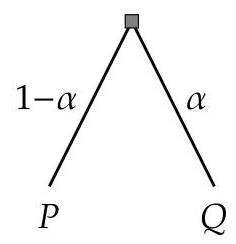
\includegraphics[width=0.3\linewidth]{images/ch05-fig02.jpg}
    \caption{将两个彩票 \(P\) 和 \(Q\) 组合成 \(\left( {1 - \alpha }\right) P + {\alpha Q}\) 的概率树。}
  \end{figure}
 

在第一阶段，以概率 \(1 - \alpha\) 选择 \(P\) ，以概率 \(\alpha\) 选择 \(Q\) ，然后以各自的结果概率来进行所选的彩票(和往常一样，不同的随机机会行动是相互独立的)。如果这些结果是 \({x}_{i}\) ，在 \(P\) 下的概率为 \({p}_{i}\) ，在 \(Q\) 下的概率为 \({q}_{i}\) ，对于 \(1 \leq  i \leq  n\) ，那么组合彩票 \(\left( {1 - \alpha }\right) P + {\alpha Q}\) 也可以被视为一个单阶段过程，以概率 \(\left( {1 - \alpha }\right) {p}_{i} + \alpha {q}_{i}\) 选择 \({x}_{i}\) ，对于 \(1 \leq  i \leq  n\) ，因此它是通常意义上的彩票。

我们总是将组合彩票写为 \(\left( {1 - \alpha }\right) P + {\alpha Q}\) ，这样概率 \(\alpha\) 选择第二个彩票 \(Q\) ，因为对于 \(\alpha  \in  \left\lbrack  {0,1}\right\rbrack\) ，情况 \(\alpha  = 0\) 作为区间 \(\left\lbrack  {0,1}\right\rbrack\) 的左端点自然对应于(5.15)中选择 \(P\) 的左分支，而情况 \(\alpha  = 1\) 作为区间 \(\left\lbrack  {0,1}\right\rbrack\) 的右端点对应于选择 \(Q\) 的右分支。如果(像通常那样)我们将这样的组合写为 \({\beta P} + \left( {1 - \beta }\right) Q\) 对于 \(\beta  \in  \left\lbrack  {0,1}\right\rbrack\) (当然，当 \(\beta  = 1 - \alpha\) 时在数学上是等价的)，这种对应关系就会丢失。

简单彩票是一种以概率 \(1 - \alpha\) 选择结果 \(x\) ，以概率 \(\alpha\) 选择结果 \(y\) 的彩票，我们用 \(x{ \land  }_{\alpha }y\) 表示(就像一个小概率树)。回想一下，选择确定结果 \(x\) 的彩票写为 \({\mathbf{1}}_{x}\) ，因此根据定义

\begin{equation}
\label{eq:5.16}
x{ \land  }_{\alpha }y = \left( {1 - \alpha }\right) {\mathbf{1}}_{x} + \alpha {\mathbf{1}}_{y}.
\end{equation}

注意，简单彩票 \(x{ \land  }_{\alpha }y\) 是一种有一个或两个结果的彩票(如果 \(x = y\) 或者 \(\alpha  = 0\) 或者 \(\alpha  = 1\) ，则它只有一个结果)。显然，

\begin{equation}
\label{eq:5.17}
\mathbb{E}\left( {u,x{ \land  }_{\alpha }y}\right)  = \left( {1 - \alpha }\right) u\left( x\right)  + {\alpha u}\left( y\right) .
\end{equation}

在下面的命题中，我们假设参与人对简单彩票的偏好由他们对函数 \(u : X \rightarrow  \mathbb{R}\) 的期望值来表示，如(5.1)和(5.17)所示，我们将其称为“简单彩票的期望效用函数”。该命题表明， \(u\) 在尺度等价意义下是唯一的。一旦参与人对简单彩票的偏好 \(\precsim\) 以这种方式确定，他对一般彩票的偏好就会自动确定(前提是它满足我们稍后会考虑的某些假设)。

命题 5.2。设 \(S\) 是 \(\Delta \left( X\right)\) 的一个包含所有简单彩票的子集。设 \(u : X \rightarrow  \mathbb{R}\) 是一个对所有 \(P,Q \in  S\) 都满足(5.1)的函数。那么，如果 \(v\) 是另一个这样的函数，则 \(u\) 和 \(v\) 是尺度等价的，即，对于某些 \(a,b\) 且对于所有 \(x \in  X\) 有 \(a > 0\) ，(5.12)成立。

证明。在这个证明中，设“效用函数”是一个对所有简单彩票 \(P,Q \in  S\) 都满足(5.1)的函数 \(u\) 。考虑一个给定的效用函数 \(\widehat{u} : X \rightarrow  \mathbb{R}\) 。如果决策者对所有结果无差异，因此对所有彩票也无差异，那么任何效用函数都是常数，并且所有效用函数都是尺度等价的(通过添加合适的常数)。因此，我们可以假设存在两个结果 \({x}_{0}\) 和 \({x}_{1}\) ，使得 \({x}_{0} \prec  {x}_{1}\) ，从而 \(\widehat{u}\left( {x}_{0}\right)  < \widehat{u}\left( {x}_{1}\right)\) 。定义函数 \(u : X \rightarrow  \mathbb{R}\) 为

\[
u\left( x\right)  = \frac{1}{\widehat{u}\left( {x}_{1}\right)  - \widehat{u}\left( {x}_{0}\right) }\widehat{u}\left( x\right)  - \frac{\widehat{u}\left( {x}_{0}\right) }{\widehat{u}\left( {x}_{1}\right)  - \widehat{u}\left( {x}_{0}\right) }
\]

这是一个与 \(\widehat{u}\) 尺度等价且满足

\begin{equation}
\label{eq:5.18}
u\left( {x}_{0}\right)  = 0,\;u\left( {x}_{1}\right)  = 1.
\end{equation}

我们证明任何其他效用函数 \(v : X \rightarrow  \mathbb{R}\) 都与 \(u\) 尺度等价，通过

\begin{equation}
\label{eq:5.19}
v\left( x\right)  = {au}\left( x\right)  + b\;\text{ with }\;a = v\left( {x}_{1}\right)  - v\left( {x}_{0}\right) ,\;b = v\left( {x}_{0}\right) .
\end{equation}

这里， \(a\) 和 \(b\) 由(5.18)唯一确定，并且

\begin{equation}
\label{eq:5.20}
v\left( {x}_{0}\right)  = {au}\left( {x}_{0}\right)  + b,\;v\left( {x}_{1}\right)  = {au}\left( {x}_{1}\right)  + b.
\end{equation}

考虑任何结果 \(z\) 。那么以下三种情况之一适用:

\begin{equation}
\label{eq:5.21}
z \prec  {x}_{0},\;{x}_{0} \precsim  z \precsim  {x}_{1},\;\text{ or }\;{x}_{1} \prec  z.
\end{equation}

我们首先考虑(5.21)中的中间情况 \({x}_{0} \lesssim  z \lesssim  {x}_{1}\) 。那么 \(0 = u\left( {x}_{0}\right)  \leq  u\left( z\right)  \leq\)  \(u\left( {x}_{1}\right)  = 1\) 。设 \(\alpha  = u\left( z\right)\) ，并考虑简单彩票 \(P = {x}_{0}{ \land  }_{\alpha }{x}_{1}\) ，使得根据(5.17)

\[
\mathbb{E}\left( {u,P}\right)  = \mathbb{E}\left( {u,{x}_{0}{ \land  }_{\alpha }{x}_{1}}\right)  = \left( {1 - \alpha }\right) u\left( {x}_{0}\right)  + {\alpha u}\left( {x}_{1}\right)  = \alpha  = u\left( z\right)
\]

因此 \(z \sim  P\) 。效用函数 \(v\) 表示相同的无差异，因此根据(5.20)和(5.18)

\[
v\left( z\right)  = \mathbb{E}\left( {v,P}\right)  = \mathbb{E}\left( {v,{x}_{0}{ \land  }_{\alpha }{x}_{1}}\right)
\]

\[
= \left( {1 - \alpha }\right) v\left( {x}_{0}\right)  + {\alpha v}\left( {x}_{1}\right)
\]

\[
= \left( {1 - \alpha }\right) \left( {{au}\left( {x}_{0}\right)  + b}\right)  + \alpha \left( {{au}\left( {x}_{1}\right)  + b}\right)
\]

\[
= \alpha  \cdot  a + b = {au}\left( z\right)  + b
\]

这表明对于 \(x = z\) (5.19)成立。

接下来，考虑情况 \(z \prec  {x}_{0}\) ，这种情况类似但稍微复杂一些。因为 \(z \prec  {x}_{0} \prec  {x}_{1}\) ，我们现在选择一个简单彩票 \(Q = z{ \land  }_{\beta }{x}_{1}\) ，使得 \(Q \sim  {x}_{0}\) ，即，

\[
\left( {1 - \beta }\right) u\left( z\right)  + {\beta u}\left( {x}_{1}\right)  = u\left( {x}_{0}\right)
\]

如果 \(\beta \left( {u\left( {x}_{1}\right)  - u\left( z\right) }\right)  = u\left( {x}_{0}\right)  - u\left( z\right)\) 或 \(\beta  = \frac{-u\left( z\right) }{1 - u\left( z\right) } = 1 - \frac{1}{1 - u\left( z\right) }\) 成立，则该式成立，其中 \(0 < \beta  < 1\) ，因为 \(u\left( z\right)  < u\left( {x}_{0}\right)  = 0\) 。此外，

\begin{equation}
\label{eq:5.22}
u\left( z\right)  = \frac{-\beta }{1 - \beta }.
\end{equation}

因为 \(Q \sim  {x}_{0}\) ，我们有

\[
\mathbb{E}\left( {v,Q}\right)  = v\left( {x}_{0}\right)
\]

\[
\left( {1 - \beta }\right) v\left( z\right)  + {\beta v}\left( {x}_{1}\right)  = v\left( {x}_{0}\right)
\]

\[
\left( {1 - \beta }\right) v\left( z\right)  + \beta \left( {{au}\left( {x}_{1}\right)  + b}\right)  = {au}\left( {x}_{0}\right)  + b
\]

\[
\left( {1 - \beta }\right) v\left( z\right)  + \beta \left( {a + b}\right)  = b
\]

\[
\left( {1 - \beta }\right) v\left( z\right)  =  - {\beta a} + \left( {1 - \beta }\right) b
\]

\begin{equation}
\label{eq:5.23}
v\left( z\right)  = \frac{-\beta }{1 - \beta }a + b = {au}\left( z\right)  + b
\end{equation}

这表明，如果 \(z \prec  {x}_{0}\) ，则对于 \(x = z\) 有 (5.19) 式成立。(5.21) 中的第三种情况 \({x}_{1} \prec  z\) 是类似的，通过选择一个简单彩票 \({x}_{0}{ \land  }_{\gamma }z\) ，使得参与人对该彩票和 \({x}_{1}\) 无差异，然后再次使用 (5.20) 式(见练习~\ref{exer:5.2})。这就证明了该命题。

命题 5.2 的证明凸显了效用函数值的含义:考虑两个结果 \({x}_{0}\) 和 \({x}_{1}\) ，使得 \({x}_{0} \prec  {x}_{1}\) 。首先，效用函数 \(u\) 总是可以进行缩放，使得如 (5.18) 式所示，效用尺度的原点为 \(u\left( {x}_{0}\right)  = 0\) ，并以 \(u\left( {x}_{1}\right)  - u\left( {x}_{0}\right)  = 1\) 确定效用单位。其次，考虑某个结果 \(z\) ，使得 \({x}_{0} \prec  z \prec  {x}_{1}\) 。这个条件表明存在某个概率 \(\alpha\) ，使得参与人对 \(z\) 和简单彩票 \({x}_{0}{ \land  }_{\alpha }{x}_{1}\) 无差异。也就是说，我们有等价的表述

\[
z \sim  {x}_{0}{ \land  }_{\alpha }{x}_{1},\;u\left( z\right)  = \left( {1 - \alpha }\right) u\left( {x}_{0}\right)  + {\alpha u}\left( {x}_{1}\right) ,
\]

和

\begin{equation}
\label{eq:5.24}
\alpha  = \frac{u\left( z\right)  - u\left( {x}_{0}\right) }{u\left( {x}_{1}\right)  - u\left( {x}_{0}\right) }
\end{equation}

其中根据 (5.18) 式有 \(\alpha  = u\left( z\right)\) 。换句话说，对于介于较不偏好和较偏好结果 \({x}_{0}\) 和 \({x}_{1}\) 之间的结果 \(z\) ，其效用 \(u\left( z\right)\) 就是在简单彩票 \({x}_{0}{ \land  }_{\alpha }{x}_{1}\) 中获得较偏好结果 \({x}_{1}\) 的概率，假设采用了 (5.18) 式的缩放方式。如果不进行这种缩放， \(\alpha\) 就是更一般的商 (5.24) ，这是基于以下观察得到的:对于任意实数 \(A,B,C\) ，且 \(A < C\) ，

\begin{equation}
\label{eq:5.25}
A < B < C,\;B = \left( {1 - \alpha }\right) A + {\alpha C}\; \Leftrightarrow  \;\alpha  = \frac{B - A}{C - A},\;0 < \alpha  < 1.
\end{equation}

选取两个结果 \({x}_{0}\) 和 \({x}_{1}\) ，并确定概率 \(\alpha\) ，使得 \(z \sim  {x}_{0}{ \land  }_{\alpha }{x}_{1}\) 成为一种为满足 \({x}_{0} \prec  z \prec  {x}_{1}\) 的结果 \(z\) 构建效用函数 \(u\) 的值 \(u\left( z\right)\) 的可能方法。如果 \({x}_{0}\) 是所有结果中最不受偏好的结果，而 \({x}_{1}\) 是最受偏好的结果，那么这将唯一地确定效用函数(即如果 \(z \sim  {x}_{0}\) 则 \(u\left( z\right)  = u\left( {x}_{0}\right)\) ，如果 \(z \sim  {x}_{1}\) 则 \(u\left( z\right)  = u\left( {x}_{1}\right)\) )。然而，即使存在这样的极端结果(例如，如果 \(X\) 是有限的)，在实践中它们对于构建效用函数可能并不那么有用，因为参与人可能不愿意考虑在最差和最好的可能结果之间进行简单彩票选择。更现实的结果 \({x}_{0}\) 和 \({x}_{1}\) 通常更有用。这就引出了 (5.21) 中的其他情况 \(z \prec  {x}_{0}\) 和 \({x}_{1} \prec  z\) ，在这种情况下，可以像命题 5.2 的证明中那样构建其他简单彩票。然后使用该彩票中的概率，通过一般表达式 (5.24) 来找到未知的效用值 \(u\left( z\right)\) ，但要根据参与人对 \(z\) 相对于 \({x}_{0}\) 和 \({x}_{1}\) 的偏好来交换结果 \(z,{x}_{0},{x}_{1}\) 的角色。

总之，如果一个期望效用函数能表示参与人对简单彩票(即有两个结果，第二个结果的概率为任意 \(\alpha\) ，第一个结果的概率为 \(1 - \alpha\) 的彩票)的偏好，那么它在正仿射变换下是唯一的。找到一个合适的 \(\alpha\) ，使得参与人对该彩票和另一个结果无差异，就可以用来构建效用函数。然后，该效用函数可用于确定参与人对更复杂彩票的偏好。

接下来，我们将只考虑彩票之间的偏好以及这种偏好的某些一致性公理。然后我们将证明，满足这些公理的偏好关系可以用一个期望效用函数来表示。

\section{ 一致性公理}

考虑结果集 \(X\) 上的彩票集 \(\Delta \left( X\right)\) 上的偏好关系 \(\precsim\) ，以及它在 (5.4) 和 (5.5) 中导出的关系 \(\sim\) 和 \(\prec\) 。为了证明 \(\precsim\) 可以根据 (5.1) 用一个期望效用函数来表示，我们考虑一些充分假设，并将其称为公理。这些是关于参与人偏好应当满足何种形式的合理规范性条件。

第一个条件，已在 (5.7) 和 (5.9) 中陈述，即 \(\precsim\) 是完全的且具有传递性。如前所述，这是一个有用的规范假设，因为否则参与人有时将无法下定决心；这可能导致任意选择和事实上的无差异，而这通常不是预期的情况。

以下关于 \(\precsim\) 的条件会影响如 (5.15) 中彩票的组合。首先，假设只有每个结果的最终概率重要，而这些概率是否来自多阶段过程并不重要。

设 \(P,Q,R\) 为彩票， \(\alpha\) 为概率。以下条件表明，当彩票被代入其他彩票时，彩票之间的无差异关系得以保留:

\begin{equation}
\label{eq:5.26}
P \sim  Q\; \Rightarrow  \;\left( {1 - \alpha }\right) R + {\alpha P} \sim  \left( {1 - \alpha }\right) R + {\alpha Q}.
\end{equation}

这里，参与人对 \(P\) 和 \(Q\) 无差异，并且如果这些彩票以某个概率 \(\alpha\) 出现在一个组合彩票中，而该组合彩票在其他情况下选择另一个彩票 \(R\) ，参与人仍然保持无差异。类似的条件对于严格偏好也成立，其中需要 \(\alpha  > 0\) :

\begin{equation}
\label{eq:5.27}
P \prec  Q,\;0 < \alpha  \leq  1\; \Rightarrow  \;\left( {1 - \alpha }\right) R + {\alpha P} \prec  \left( {1 - \alpha }\right) R + {\alpha Q}.
\end{equation}

条件(5.26)和(5.27)也称为无关备选方案独立性，或简称为独立性公理。这里的“无关备选方案”是彩票 \(R\) ：它不应影响无差异关系 \(P \sim  Q\) 或严格偏好关系 \(P \prec  Q\) 。
  \begin{figure}[H]
    \centering
    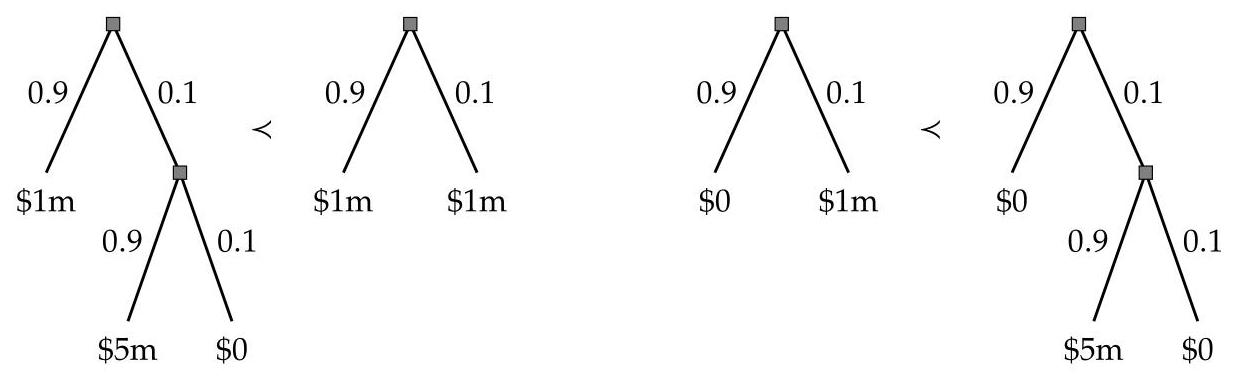
\includegraphics[width=0.6\linewidth]{images/ch05-fig03.jpg}
    \caption{阿莱悖论中的彩票组合。}
    \label{fig:5.2}
  \end{figure}
  
图~\ref{fig:5.2}展示了阿莱悖论，这是条件(5.27)的一个经验反例，涉及三种假设结果 \(x,y,z\) ，即获得100万美元、500万美元或0美元， \(P = y{ \land  }_{0.1}z\) 和 \(Q = {\mathbf{1}}_{x}\) ，其中 \(R\) 可以是 \({\mathbf{1}}_{x}\) 或 \({\mathbf{1}}_{z}\) 。

图~\ref{fig:5.2}给出了一个被称为阿莱悖论的例子，在某些假设情形下，人们可能会违背条件(5.27)。考虑三种结果 \(x,y,z\) ，其中 \(x\) 表示“获得100万美元”， \(y\) 表示“获得500万美元”， \(z\) 表示“获得0美元”。设 \(P\) 为简单彩票 \(y{ \land  }_{0.1}z\) ，并设 \(Q = {\mathbf{1}}_{x}\) 。偏好关系 \(P \prec  Q\) 意味着参与人宁愿确定地获得100万美元，也不愿以90\%的概率获得500万美元，否则一无所获，这可能是参与人的选择。现在考虑彩票 \(R = {\mathbf{1}}_{z}\) ，并设 \(\alpha  = {0.1}\) 。那么，图~\ref{fig:5.2}右侧所示的组合彩票 \(\left( {1 - \alpha }\right) R + {\alpha P}\) 意味着参与人有91\%的概率一无所获，有9\%的概率获得500万美元；而 \(\left( {1 - \alpha }\right) R + {\alpha Q}\) 意味着参与人有90\%的概率一无所获，有10\%的概率获得100万美元。鉴于参与人很可能无论如何都一无所获，他的偏好现在可能会逆转，即 \(\left( {1 - \alpha }\right) R + {\alpha Q} \prec  \left( {1 - \alpha }\right) R + {\alpha P}\) ，这与条件(5.27)相矛盾。另一方面，如果是图~\ref{fig:5.2}左侧所示的 \(R = {\mathbf{1}}_{x}\) ，那么 \(\left( {1 - \alpha }\right) R + {\alpha P}\) 意味着参与人有90\%的概率获得100万美元，有1\%的概率一无所获，有9\%的概率获得500万美元；而 \(\left( {1 - \alpha }\right) R + {\alpha Q}\) 意味着参与人确定地获得100万美元，这很可能使他在与 \(R\) 组合时也保持原来的偏好 \(P \prec  Q\) ，符合条件(5.27)。

为解决图~\ref{fig:5.2}中违背条件(5.27)的不一致偏好问题，建议的解决办法是，参与人应该:(a)确定自己的偏好是 \(P \prec  Q\) 还是 \(Q \prec  P\) (或者 \(P \sim  Q\) )，这需要忽略无关备选方案 \({\mathbf{1}}_{z}\) 或 \({\mathbf{1}}_{x}\) ；(b)考虑当彩票 \(P = {\mathbf{1}}_{z}{ \land  }_{0.9}{\mathbf{1}}_{y}\) 中出现不理想的结果 \({\mathbf{1}}_{z}\) 时，自己应给予后悔(后悔)情绪多大的权重，以及在图~\ref{fig:5.2}中他偏好的组合彩票 \(\left( {1 - \alpha }\right) {\mathbf{1}}_{z} + {\alpha P}\) 中这种后悔情绪“不可见”是否重要。如果后悔情绪很重要，那么它应该成为结果 \(z\) 的一部分，此时结果 \(z\) 有两种形式:“本可以获得100万美元却只得到0美元”和“得到0美元，但这本来就是很可能出现的结果”。总之，图~\ref{fig:5.2}中的不一致情况在实践中很可能会出现，但独立性公理(5.27)可以通过强调基本决策应在 \(P\) 和 \(Q\) 之间进行，来帮助解决这一问题。

(5.27)的一个推论是以下相当自然的单调性性质，该性质表明，增加组合彩票中更受偏好部分 \(Q\) 的概率会使该组合彩票更受偏好。

引理5.3。考虑 \(\Delta \left( X\right)\) 上满足(5.27)的偏好关系 \(\precsim\) 。那么对于 \(\Delta \left( X\right)\) 中的 \(P,Q\) ，

\begin{equation}
\label{eq:5.28}
P \prec  Q,\;0 \leq  \alpha  < \beta  \leq  1\; \Rightarrow  \;\left( {1 - \alpha }\right) P + {\alpha Q} \prec  \left( {1 - \beta }\right) P + {\beta Q}.
\end{equation}

证明。设 \(P \prec  Q\) 和 \(0 \leq  \alpha  < \beta  \leq  1\) ，这意味着 \(0 \leq  \frac{\alpha }{\beta } < 1\) ，因此 \(0 < 1 - \frac{\alpha }{\beta } \leq  1\) 。以下概率树说明了该证明过程:
  \begin{figure}[H]
    \centering
    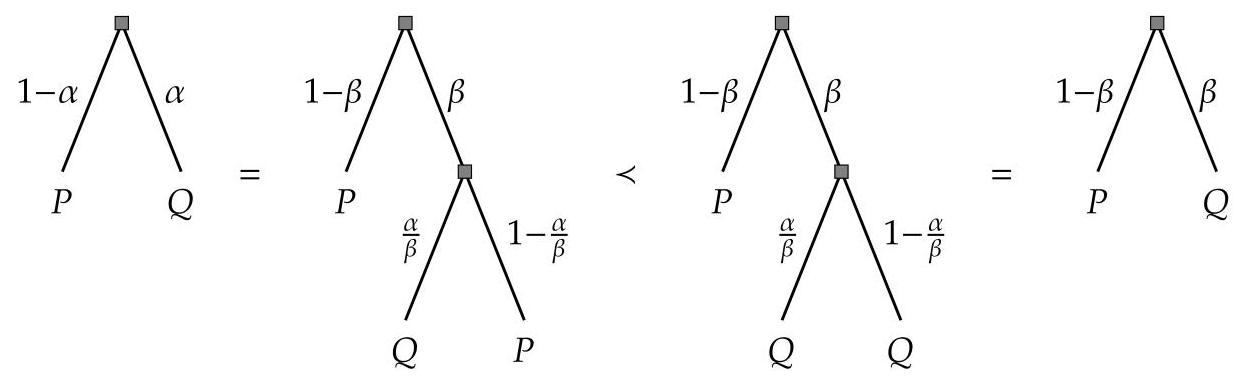
\includegraphics[width=0.6\linewidth]{images/ch05-fig04.jpg}
    \caption{}
  \end{figure}


我们两次使用(5.27)，首先证明 \(\frac{\alpha }{\beta }Q + \left( {1 - \frac{\alpha }{\beta }}\right) P \prec  \frac{\alpha }{\beta }Q + \left( {1 - \frac{\alpha }{\beta }}\right) Q\) ，然后在 \(\left( {1 - \beta }\right) P + \beta {Q}^{\prime }\) 中用任一组合彩票替换 \({Q}^{\prime }\) ，这就证明了(5.28)。

下一个条件称为连续性公理，其中 \(P,Q,R\) 是彩票， \(\alpha\) 是一个概率:

\begin{equation}
\label{eq:5.29}
P \prec  Q \prec  R\; \Rightarrow  \;\exists \alpha  \in  \left( {0,1}\right)  : Q \sim  \left( {1 - \alpha }\right) P + {\alpha R}.
\end{equation}

为了理解为什么条件(5.29)可能被认为有问题，设 \(P\) 为“在接下来的一分钟内死亡”， \(Q\) 为“一无所获”， \(R\) 为“获得一美元”。那么 \(Q \sim  \left( {1 - \alpha }\right) P + {\alpha R}\) 意味着参与人会以正概率 \(1 - \alpha\) 冒生命危险，只是为了以概率 \(\alpha\) 获得一美元，这似乎不合理。对此的反驳观点是，只要 \(1 - \alpha\) 为正，它可以任意小，例如 \({2}^{-{500}}\) ，就像一枚公平的硬币连续500次都掷出“正面”一样。这是极小的风险，而且人们确实会为了小收益而以小概率冒生命危险，例如骑自行车不戴头盔。条件(5.29)是一个技术性限制，而非实际限制。

当偏好 \(<\) 由期望效用函数 \(u\) 表示时，连续性公理(5.29)必然成立，因为 \(P \prec  Q \prec  R\) 意味着 \(\mathbb{E}\left( {u,P}\right)  < \mathbb{E}\left( {u,Q}\right)  < \mathbb{E}\left( {u,R}\right)\) ，所以根据(5.25)，当 \(\alpha  = \frac{\mathbb{E}\left( {u,Q}\right)  - \mathbb{E}\left( {u,P}\right) }{\mathbb{E}\left( {u,R}\right)  - \mathbb{E}\left( {u,P}\right) }\) 时，我们有 \(0 < \alpha  < 1\) 且

\begin{equation}
\label{eq:5.30}
\mathbb{E}\left( {u,Q}\right)  = \left( {1 - \alpha }\right) \mathbb{E}\left( {u,P}\right)  + \alpha \mathbb{E}\left( {u,R}\right)  = \mathbb{E}\left( {u,\left( {1 - \alpha }\right) P + {\alpha R}}\right)
\end{equation}

因此 \(Q \sim  \left( {1 - \alpha }\right) P + {\alpha R}\) 。

因为效用函数 \(u : X \rightarrow  \mathbb{R}\) 取实数值，所以存在具有偏好关系 \(\lesssim\) 的集合 \(X\) (已限制为确定性结果)，根据(5.8)不能用效用函数来表示。经典的例子是 \(X = {\left\lbrack  0,1\right\rbrack  }^{2}\) 与 \(\precsim\) 构成的字典序 \({ \leq  }_{\text{ lex }}\) ，如(5.11)所定义，如图5.3所示。
  \begin{figure}[H]\label{fig:5.3}
    \centering
    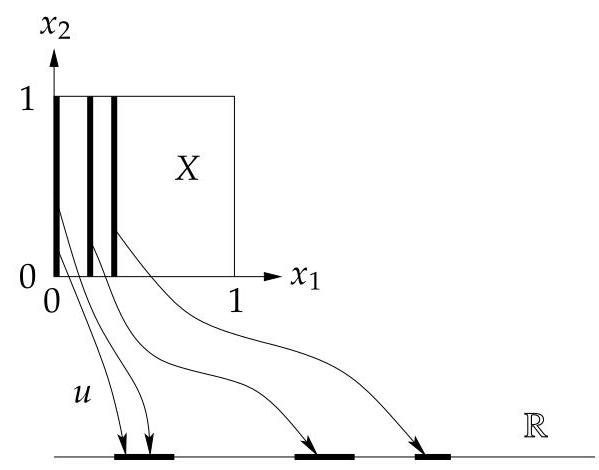
\includegraphics[width=0.6\linewidth]{images/ch05-fig05.jpg}
    \caption{集合 \(X = {\left\lbrack  0,1\right\rbrack  }^{2}\) ，其字典序为 \({ \leq  }_{\text{ lex }}\) ，以 \(\precsim\) 表示。一个效用函数 \(u\left( {{x}_{1},{x}_{2}}\right)\) 必须将 \(X\) 中不可数的垂直条带映射到 \(\mathbb{R}\) 中的非空不相交区间，这是不可能的。}
  \end{figure}


假设存在一个效用函数 \(u : {\left\lbrack  0,1\right\rbrack  }^{2} \rightarrow  \mathbb{R}\) ，使得根据式(5.11)，

\[
\left( {{x}_{1},{x}_{2}}\right)  \prec  \left( {{y}_{1},{y}_{2}}\right)  \Leftrightarrow  \left( {{x}_{1},{x}_{2}}\right) { \leq  }_{\text{ lex }}\left( {{y}_{1},{y}_{2}}\right) \;\text{ and }\;\left( {{x}_{1},{x}_{2}}\right)  \neq  \left( {{y}_{1},{y}_{2}}\right)
\]

\[
\Leftrightarrow  {x}_{1} < {y}_{1}\;\text{ or }\;\left( {{x}_{1} = {y}_{1}\text{ and }{x}_{2} < {y}_{2}}\right)
\]

\begin{equation}
\label{eq:5.31}
\Leftrightarrow  u\left( {{x}_{1},{x}_{2}}\right)  < u\left( {{y}_{1},{y}_{2}}\right) \text{ . }
\end{equation}

现在考虑形式为 \(\left\{  {x}_{1}\right\}   \times  \left\lbrack  {0,1}\right\rbrack\) 的“垂直条带”，它是 \(X\) 的一个子集，图5.3中用粗线展示了其中三条。对于这样一个条带上的任意两点 \(\left( {{x}_{1},{x}_{2}}\right)\) 和 \(\left( {{x}_{1},{y}_{2}}\right)\) ，使得 \({x}_{2} < {y}_{2}\) (例如，端点 \(\left( {{x}_{1},0}\right)\) 和 \(\left( {{x}_{1},1}\right)\) )，我们有 \(u\left( {{x}_{1},{x}_{2}}\right)  < u\left( {{x}_{1},{y}_{2}}\right)\) 。对于两个这样的条带 \(\left\{  {x}_{1}\right\}   \times  \left\lbrack  {0,1}\right\rbrack\) 和 \(\left\{  {y}_{1}\right\}   \times  \left\lbrack  {0,1}\right\rbrack\) ，且 \({x}_{1} < {y}_{1}\) ，字典序要求 \(u\left( {{x}_{1},1}\right)  < u\left( {{y}_{1},0}\right)\) 。因此，这些条带在 \(u\) 下的像不能重叠，它们是 \(u\) 的值域 \(\mathbb{R}\) 中两两不相交区间的子集。如果只有有限个这样的条带(就像图中画出的具有一定宽度的条带那样)，这是可行的，但从数学角度来看，它们没有宽度，因此这些条带的像无法不相交地“放入” \(\mathbb{R}\) 中。从技术上讲，对于任意 \({x}_{1} \in  \left\lbrack  {0,1}\right\rbrack\) ，我们可以选择一个有理数 \(r\left( {x}_{1}\right)\) ，使得 \(u\left( {{x}_{1},0}\right)  < r\left( {x}_{1}\right)  < u\left( {{x}_{1},1}\right)\) 。如果 \({x}_{1} < {y}_{1}\) ，那么 \(u\left( {{x}_{1},1}\right)  < u\left( {{y}_{1},0}\right)\) ，因此 \(r\left( {x}_{1}\right)  < r\left( {y}_{1}\right)\) 。因此，映射 \({x}_{1} \mapsto  r\left( {x}_{1}\right)\) 定义了一个从集合 \(\left\lbrack  {0,1}\right\rbrack\) 到有理数集 \(\mathbb{Q}\) 的单射，这意味着 \(\left\lbrack  {0,1}\right\rbrack\) 的集合论基数至多与 \(\mathbb{Q}\) 相同。这是一个矛盾，因为 \(\mathbb{Q}\) 是可数集，而 \(\left\lbrack  {0,1}\right\rbrack\) 不是。因此，一个实值效用函数 \(u : {\left\lbrack  0,1\right\rbrack  }^{2} \rightarrow  \mathbb{R}\) 不能像式(5.31)那样表示字典序 \({ \leq  }_{\text{ lex }}\) 。

对第一个分量变化的极端“敏感性”是不将字典序规则用作偏好关系的一个数学原因。出于同样的原因，该规则在行为上也存在疑问，正如我们之前在(5.11)和(5.29)之后针对“生命安全”相对于“金钱收益”的字典序偏好所讨论的那样。

如(5.30)所示，期望效用函数的存在意味着连续性公理(5.29)。如果限制在确定性结果上的偏好 \(\lesssim\) 是 \(X = {\left\lbrack  0,1\right\rbrack  }^{2}\) 上的字典序 \({ \leq  }_{\text{ lex }}\) ，那么它违反了连续性公理，并且期望效用函数不存在。在下一节中，我们将展示连续性公理(5.29)如何用于构建期望效用函数。

\section{期望效用函数的存在性}

以下是本章的核心定理。证明的主要思路已在5.2节给出。这里给出的证明更长，因为它不假设存在最不偏好的结果 \({x}_{0}\) 和最偏好的结果 \({x}_{1}\) 。相反，可以选择任意两个结果 \({x}_{0}\) 和 \({x}_{1}\) 来定义效用函数的原点和单位。然后，可以像命题5.2那样为更多的结果 \(z\) (例如，对于 \(z \prec  {x}_{0}\) )定义效用函数。对于与 \(u\) 尺度等价且以 \(P\) 的最不偏好和最偏好结果进行缩放的函数 \(v\) (其中我们利用 \(P\) 只有有限多个结果这一事实)，期望效用性质被证明对于任意彩票 \(P\) 都成立。

定理5.4。设 \(\Delta \left( X\right)\) 是结果集 \(X\) 上的彩票集合，设 \(\precsim\) 是 \(\Delta \left( X\right)\) 上的偏好关系。假设 \(\lesssim\) 是完全的且传递的，并且满足独立性公理(5.26)和(5.27)以及连续性公理(5.29)。那么存在一个期望效用函数 \(u : X \rightarrow  \mathbb{R}\) ，它根据(5.1)表示 \(\lesssim\) 。证明。 \(\precsim\) 是完全的且传递的这一事实意味着(5.4)和(5.5)中定义的 \(\sim\) 和 \(\prec\) 也是完全的且传递的，我们一直会用到这一点，例如当将 \({x}_{0} \precsim  z \precsim  {x}_{1}\) 简写为 \({x}_{0} \precsim  z\) 和 \(z \precsim  {x}_{1}\) 时。我们将反复使用连续性公理。注意，如果如(5.29)中的 \(P \prec  Q \prec  R\) 和 \(Q \sim  \left( {1 - \alpha }\right) P + {\alpha R}\) ，那么 \(\alpha\) 是唯一的，因为如果 \(\alpha  < \beta\) ，那么根据引理5.3有 \(\left( {1 - \alpha }\right) P + {\alpha R} \prec  \left( {1 - \beta }\right) P + {\beta R}\) ，所以我们不能同时有 \(Q \sim  \left( {1 - \beta }\right) P + {\beta R}\) 。

如果参与人对所有结果都无差异，那么他对所有基于结果的彩票也无差异，此时一个常数效用函数就足够了。因此，假设存在两个结果 \({x}_{0}\) 和 \({x}_{1}\) ，使得 \({x}_{0} \prec  {x}_{1}\) 。正如在命题 5.2 的证明中那样，我们使用 \({x}_{0}\) 和 \({x}_{1}\) 来确定效用函数 \(u\) 的原点和单位，如式 (5.18) 所示，即 \(u\left( {x}_{0}\right)  = 0\) 且 \(u\left( {x}_{1}\right)  = 1\) 。对于任何结果 \(z\) ，我们随后借助一个合适的简单彩票来选择效用函数的值 \(u\left( z\right)\) :

\begin{itemize}
\item 如果 \(z \sim  {x}_{0}\) ，则令 \(u\left( z\right)  = 0\) ；如果 \(z \sim  {x}_{1}\) ，则令 \(u\left( z\right)  = 1\) 。
\end{itemize}

\begin{itemize}
\item 如果 \({x}_{0} < z < {x}_{1}\) ，则根据式 (5.29) 找到 \(\alpha\) 使得 \(z \sim  \left( {1 - \alpha }\right) {\mathbf{1}}_{{x}_{0}} + \alpha {\mathbf{1}}_{{x}_{1}} = {x}_{0}{ \land  }_{\alpha }{x}_{1}\) ，并令 \(u\left( z\right)  = \alpha\) 。
\end{itemize}

\begin{itemize}
\item 如果 \(z \prec  {x}_{0} \prec  {x}_{1}\) ，同样根据式 (5.29) 找到 \(\beta\) 使得 \({x}_{0} \sim  z{ \land  }_{\beta }{x}_{1}\) ，并如式 (5.22) 那样令 \(u\left( z\right)  = \frac{-\beta }{1 - \beta }\) 。
\end{itemize}

\begin{itemize}
\item 如果 \({x}_{0} \prec  {x}_{1} \prec  z\) ，根据式 (5.29) 找到 \(\gamma\) 使得 \({x}_{1} \sim  {x}_{0}{ \land  }_{\gamma }z\) ，并令 \(u\left( z\right)  = \frac{1}{\gamma }\) 。
\end{itemize}

在所有情况下， \(u\left( z\right)\) 由参与人对确定结果和简单彩票的无差异来确定。例如，在最后一种情况下， \(u\left( {x}_{1}\right)  = 1 =\)  \(\mathbb{E}\left( {u,{x}_{0}{ \land  }_{\gamma }z}\right)  = \left( {1 - \gamma }\right) u\left( {x}_{0}\right)  + {\gamma u}\left( z\right)  = {\gamma u}\left( z\right)\) ，从而 \(u\left( z\right)  = \frac{1}{\gamma }\) 。

以这种方式确定 \(u : X \rightarrow  \mathbb{R}\) 后，我们现在证明 \(u\) 满足 (5.1)，即 \(u\) 表示参与人在任意两个彩票 \(P\) 和 \(Q\) 之间的偏好。设 \({z}_{i}\) ( \(1 \leq  i \leq  n\) )为 \(P\) 或 \(Q\) 的结果，其中 \({z}_{i}\) 在 \(P\) 下的概率为 \({p}_{i}\) ，在 \(Q\) 下的概率为 \({q}_{i}\) 。我们首先假设所有这些结果都满足 \({x}_{0} \precsim  {z}_{i} \precsim  {x}_{1}\) 。设 \({\alpha }_{i} = u\left( {z}_{i}\right)\) ，根据 \(u\) 的构造，我们有 \({z}_{i} \sim  {x}_{0}{ \land  }_{{\alpha }_{i}}{x}_{1}\) 。现在，根据 (5.26) 依次用等价彩票替换，我们将每个结果 \({z}_{i}\) 替换为其等价彩票 \({x}_{0}{ \land  }_{{\alpha }_{i}}{x}_{1}\) 。即(见图 5.1)

\[
P = \mathop{\sum }\limits_{{i = 1}}^{n}{p}_{i}{\mathbf{1}}_{{z}_{i}} \sim  \mathop{\sum }\limits_{{i = 1}}^{n}{p}_{i}\left( {{x}_{0}{ \land  }_{{\alpha }_{i}}{x}_{1}}\right)
\]

\[
= \mathop{\sum }\limits_{{i = 1}}^{n}{p}_{i}\left( {\left( {1 - {\alpha }_{i}}\right) {\mathbf{1}}_{{x}_{0}} + {\alpha }_{i}{\mathbf{1}}_{{x}_{1}}}\right)
\]

\[
= \left( {1 - \mathop{\sum }\limits_{{i = 1}}^{n}{p}_{i}{\alpha }_{i}}\right) {\mathbf{1}}_{{x}_{0}} + \left( {\mathop{\sum }\limits_{{i = 1}}^{n}{p}_{i}{\alpha }_{i}}\right) {\mathbf{1}}_{{x}_{1}}
\]

\begin{equation}
\label{eq:5.32}
= \left( {1 - p}\right) {\mathbf{1}}_{{x}_{0}} + p{\mathbf{1}}_{{x}_{1}} = {x}_{0}{ \land  }_{p}{x}_{1}
\end{equation}

与

\begin{equation}
\label{eq:5.33}
p = \mathop{\sum }\limits_{{i = 1}}^{n}{p}_{i}{\alpha }_{i} = \mathop{\sum }\limits_{{i = 1}}^{n}{p}_{i}u\left( {z}_{i}\right)  = \mathbb{E}\left( {u,P}\right) .
\end{equation}

类似地

\begin{equation}
\label{eq:5.34}
Q \sim  {x}_{0}{ \land  }_{q}{x}_{1}\;\text{ with }\;q = \mathop{\sum }\limits_{{i = 1}}^{n}{q}_{i}{\alpha }_{i} = \mathop{\sum }\limits_{{i = 1}}^{n}{q}_{i}u\left( {z}_{i}\right)  = \mathbb{E}\left( {u,Q}\right) .
\end{equation}

推导式 (5.32) 是该论证的核心:

\begin{itemize}
\item 根据构造，结果 \({z}_{i}\) 的效用 \(u\left( {z}_{i}\right)\) 是概率 \({\alpha }_{i}\) ，使得参与人对 \({z}_{i}\) 和以概率 \({\alpha }_{i}\) 选择更好结果 \({x}_{1}\) 的简单彩票 \({x}_{0}{ \land  }_{{\alpha }_{i}}{x}_{1}\) 无差异。
\end{itemize}

\begin{itemize}
\item 在 \(P\) 中，每个结果 \({z}_{i}\) 都被其简单彩票 \({x}_{0}{ \land  }_{{\alpha }_{i}}{x}_{1}\) 替换，通过重复应用 (5.26) 得到一个同与之无差异的彩票。
\end{itemize}

\begin{itemize}
\item 最终得到的总体彩票只有两个结果 \({x}_{0}\) 和 \({x}_{1}\) ， \({x}_{1}\) 的概率为 \(p = \mathop{\sum }\limits_{{i = 1}}^{n}{p}_{i}{\alpha }_{i}\) ，因为独立独立概率可以相乘。
\end{itemize}

\begin{itemize}
\item 根据 (5.33)，\(\mathop{\sum }\limits_{{i = 1}}^{n}{p}_{i}{\alpha }_{i}\) 等于期望 \(\mathbb{E}\left( {u,P}\right)\) 。对于 \(Q\) 的相应表述是 (5.34)。
\end{itemize}

借助单调性引理5.3，我们证明 \(P \precsim  Q\) 成立当且仅当 \(\mathbb{E}\left( {u,P}\right)  \leq  \mathbb{E}\left( {u,Q}\right)\) 成立，即当且仅当 \(p \leq  q\) 成立。假设 \(P \precsim  Q\) 成立。如果 \(q < p\) 成立，那么，因为 \({x}_{0} < {x}_{1},\left( {5.28}\right)\) (其中 \({x}_{0},{x}_{1},q,p\) 对应 \(P,Q,\alpha ,\beta\) )意味着 \(Q \sim  {x}_{0}{ \land  }_{q}{x}_{1} \prec  {x}_{0}{ \land  }_{p}{x}_{1} \sim  P\) 成立，也就是 \(Q \prec  P\) 成立，这产生了矛盾。这表明 \(P \precsim  Q\) 蕴含 \(p \leq  q\) 。为了证明其逆命题，设 \(p \leq  q\) 成立。如果 \(p = q\) 成立，那么显然 \(P \sim  Q\) 成立；如果 \(p < q\) 成立，那么根据(5.28)， \(P \sim  {x}_{0}{ \land  }_{p}{x}_{1} \prec  {x}_{0}{ \land  }_{q}{x}_{1} \sim  Q\) 成立，即 \(P \prec  Q\) 成立。这表明 \(p \leq  q\) 蕴含 \(P \precsim  Q\) ，符合要求。

接下来需要证明对于彩票 \(P\) 和 \(Q\) ，(5.1) 式成立，这些彩票的结果 \({z}_{1},\ldots ,{z}_{n}\) 满足对于某些 \(i\) 有 \({z}_{i} \prec  {x}_{0}\) 或者 \({x}_{1} \prec  {z}_{i}\) 。设 \({z}_{1}\) 是所有结果 \({z}_{1},\ldots ,{z}_{n}\) 中最不被偏好的， \({z}_{n}\) 是最被偏好的。我们采用与之前相同的方法，但使用两个新的“参考结果” \({y}_{0}\) 和 \({y}_{1}\) 来代替 \({x}_{0}\) 和 \({x}_{1}\) :

\begin{itemize}
\item 如果 \({z}_{1} \prec  {x}_{0}\) 成立，那么令 \({y}_{0} = {z}_{1}\) ；否则，令 \({y}_{0} = {x}_{0}\) 。如果 \({x}_{1} \prec  {z}_{n}\) 成立，那么令 \({y}_{1} = {z}_{n}\) ；否则，令 \({y}_{1} = {x}_{1}\) 。那么对于彩票 \(P\) 和 \(Q\) 的所有结果 \({z}_{i}\) ，有 \({y}_{0} \precsim  {z}_{i} \precsim  {y}_{1}\) 成立。
\end{itemize}

\begin{itemize}
\item 定义函数 \(v : X \rightarrow  \mathbb{R}\) 如下
\end{itemize}

\[
v\left( x\right)  = \frac{u\left( x\right)  - u\left( {y}_{0}\right) }{u\left( {y}_{1}\right)  - u\left( {y}_{0}\right) },
\]

该函数与 \(u\) 是尺度等价的，并且满足

\[
v\left( {y}_{0}\right)  = 0,\;v\left( {y}_{1}\right)  = 1.
\]

\begin{itemize}
\item 用 \({y}_{0}\) 和 \({y}_{1}\) 之间的一个等偏好简单彩票来替换每个结果 \({z}_{i}\) ，对于某个概率 \({\beta }_{i}\) (这是可行的，因为 \({y}_{0} \precsim  {z}_{i} \precsim  {y}_{1}\) )
\end{itemize}

\begin{equation}
\label{eq:5.35}
{z}_{i} \sim  {y}_{0}{ \land  }_{{\beta }_{i}}{y}_{1}\;\left( {1 \leq  i \leq  n}\right) .
\end{equation}

\begin{itemize}
\item 在 \(P\) 和 \(Q\) 中，使用(5.26)式反复替换结果 \({z}_{i}\) 为(5.35)式中的简单彩票。然后，参与人对于 \(P\) 和一个具有两个结果 \({y}_{0}\) 和 \({y}_{1}\) 的合适简单彩票是无差异的，对于 \(Q\) 也是类似的。
\end{itemize}

\[
P \sim  {y}_{0}{ \land  }_{\widehat{p}}{y}_{1},\;\widehat{p} = \mathop{\sum }\limits_{{i = 1}}^{n}{p}_{i}{\beta }_{i},\;Q \sim  {y}_{0}{ \land  }_{\widehat{q}}{y}_{1},\;\widehat{q} = \mathop{\sum }\limits_{{i = 1}}^{n}{q}_{i}{\beta }_{i}.
\]

那么，如果我们能证明

\begin{equation}
\label{eq:5.36}
{\beta }_{i} = v\left( {z}_{i}\right) \;\left( {1 \leq  i \leq  n}\right)
\end{equation}

这意味着如 (5.33) 和 (5.34) 中的 \(\widehat{p} = \mathbb{E}\left( {v,P}\right)\) 和 \(\widehat{q} = \mathbb{E}\left( {v,Q}\right)\) ，我们如前所述证明当且仅当 \(\widehat{p} \leq  \widehat{q}\) 时 \(P \precsim  Q\) 。这表明 \(v\) 是一个期望效用函数，尺度等价的函数 \(u\) 也是。

概率 \({\beta }_{i}\) 由无差异条件(无差异条件)(5.35) 唯一确定，但我们不能假设 (5.36) 成立，因为 \(v\) 尽管与 \(u\) 尺度等价，但尚未被证明是一个期望效用函数，因为我们还没有针对 \(u\) 证明这一点(对于某些 \(i\) 有 \({z}_{i} \prec  {x}_{0}\) 或 \({x}_{1} \prec  {z}_{i}\) 的一般情况)。

因此，仍需证明 (5.36)。我们利用 (5.26)，借助涉及 \({y}_{0},{x}_{0},{x}_{1},{y}_{1}\) 和 \({z}_{i}\) (对于 \(1 \leq  i \leq  n\) )的简单彩票之间的合适无差异关系来完成这一点，使用 \(u\left( {z}_{i}\right)\) 的定义。计算过程是仿射变换(仿射变换)的直接应用，但有些冗长。

目标是将所有的 \({z}_{1},\ldots ,{z}_{n},{x}_{0},{x}_{1}\) 表示为 \({y}_{0}\) 和 \({y}_{1}\) 之间的简单彩票。我们首先对 \({x}_{0}\) 和 \({x}_{1}\) 进行此操作，其中

\begin{equation}
\label{eq:5.37}
{x}_{0} \sim  {y}_{0}{ \land  }_{{\eta }_{0}}{y}_{1},\;{x}_{1} \sim  {y}_{0}{ \land  }_{{\eta }_{1}}{y}_{1},
\end{equation}

我们声称

\begin{equation}
\label{eq:5.38}
{\eta }_{0} = v\left( {x}_{0}\right)  = \frac{-u\left( {y}_{0}\right) }{u\left( {y}_{1}\right)  - u\left( {y}_{0}\right) },\;{\eta }_{1} = v\left( {x}_{1}\right)  = \frac{1 - u\left( {y}_{0}\right) }{u\left( {y}_{1}\right)  - u\left( {y}_{0}\right) }.
\end{equation}

为了证明 (5.38)，我们有 \({y}_{0} \precsim  {x}_{0} \prec  {x}_{1}\) ，因此

\begin{equation}
\label{eq:5.39}
{x}_{0} \sim  {y}_{0}{ \land  }_{\beta }{x}_{1},\;u\left( {y}_{0}\right)  = \frac{-\beta }{1 - \beta }
\end{equation}

根据 \(u\left( {y}_{0}\right)\) 的构造(如果 \({y}_{0} = {x}_{0}\) 也适用，其中 \(\beta  = 0\) )。因此，通过将符号表示(5.16)明显扩展到彩票(彩票)组合，我们有

\[
{x}_{0} \sim  {y}_{0}{ \land  }_{\beta }{x}_{1} \sim  {y}_{0}{ \land  }_{\beta }\left( {{y}_{0}{ \land  }_{{\eta }_{1}}{y}_{1}}\right)  = {y}_{0}{ \land  }_{{\eta }_{0}}{y}_{1}
\]

这表明

\begin{equation}
\label{eq:5.40}
{\eta }_{0} = \beta {\eta }_{1}.
\end{equation}

同样，利用 \({x}_{0} \prec  {x}_{1} \precsim  {y}_{1}\) 和 \(u\left( {y}_{1}\right)\) 的构造

\begin{equation}
\label{eq:5.41}
{x}_{1} \sim  {x}_{0}{ \land  }_{\gamma }{y}_{1},\;u\left( {y}_{1}\right)  = \frac{1}{\gamma }
\end{equation}

(如果 \({y}_{1} = {x}_{1}\) 也适用，其中 \(\gamma  = 1\) )。因此，

\[
{x}_{1} \sim  {x}_{0}{ \land  }_{\gamma }{y}_{1} \sim  \left( {{y}_{0}{ \land  }_{{\eta }_{0}}{y}_{1}}\right) { \land  }_{\gamma }{y}_{1} = {y}_{0}{ \land  }_{{\eta }_{1}}{y}_{1}
\]

这表明

\begin{equation}
\label{eq:5.42}
{\eta }_{1} = \left( {1 - \gamma }\right) {\eta }_{0} + \gamma
\end{equation}

我们用 \(\beta\) 和 \(\gamma\) 来求解(5.40)和(5.42)中的 \({\eta }_{0}\) 和 \({\eta }_{1}\) ，即

\[
{\eta }_{1} = \left( {1 - \gamma }\right) \beta {\eta }_{1} + \gamma ,\;{\eta }_{1} = \frac{\gamma }{1 - \left( {1 - \gamma }\right) \beta },
\]

这与(5.38)中 \({\eta }_{1}\) 的表达式一致，因为根据(5.39)和(5.41)

\[
\frac{1 - u\left( {y}_{0}\right) }{u\left( {y}_{1}\right)  - u\left( {y}_{0}\right) } = \frac{1 + \frac{\beta }{1 - \beta }}{\frac{1}{\gamma } + \frac{\beta }{1 - \beta }} = \frac{\gamma \left( {1 - \beta }\right)  + {\gamma \beta }}{1 - \beta  + {\gamma \beta }} = \frac{\gamma }{1 - \left( {1 - \gamma }\right) \beta }.
\]

此外，根据(5.40)

\[
\frac{-u\left( {y}_{0}\right) }{u\left( {y}_{1}\right)  - u\left( {y}_{0}\right) } = \frac{\frac{\beta }{1 - \beta }}{\frac{1}{\gamma } + \frac{\beta }{1 - \beta }} = \frac{\gamma \beta }{1 - \beta  + {\gamma \beta }} = \beta {\eta }_{1} = {\eta }_{0}
\]

这表明了(5.38)。

为了证明(5.36)，我们对 \({z}_{i}\) 进行通常的情况区分。首先，如果 \({x}_{0} \precsim  {z}_{i} \precsim  {x}_{1}\) ，那么 \({z}_{i} \sim  {x}_{0}{ \land  }_{{\alpha }_{i}}{x}_{1}\) 且 \(u\left( {z}_{i}\right)  = {\alpha }_{i}\) 。我们代入(5.37)并得到

\[
{z}_{i} \sim  {x}_{0}{ \land  }_{{\alpha }_{i}}{x}_{1} \sim  \left( {{y}_{0}{ \land  }_{{\eta }_{0}}{y}_{1}}\right) { \land  }_{{\alpha }_{i}}\left( {{y}_{0}{ \land  }_{{\eta }_{1}}{y}_{1}}\right)  = {y}_{0}{ \land  }_{{\beta }_{i}}{y}_{1}
\]

这表明

\[
{\beta }_{i} = \left( {1 - {\alpha }_{i}}\right) {\eta }_{0} + {\alpha }_{i}{\eta }_{1} = {\eta }_{0} + {\alpha }_{i}\left( {{\eta }_{1} - {\eta }_{0}}\right)  = {\eta }_{0} + u\left( {z}_{i}\right) \left( {{\eta }_{1} - {\eta }_{0}}\right)
\]

\begin{equation}
\label{eq:5.43}
= \frac{-u\left( {y}_{0}\right) }{u\left( {y}_{1}\right)  - u\left( {y}_{0}\right) } + u\left( {z}_{i}\right) \frac{1}{u\left( {y}_{1}\right)  - u\left( {y}_{0}\right) } = v\left( {z}_{i}\right) ,
\end{equation}

这再次表明了(5.36)。

如果 \({y}_{0} \precsim  {z}_{i} \prec  {x}_{0}\) ，那么根据 \(u\left( {z}_{i}\right)\) 的构造，我们有 \({x}_{0} \sim  {z}_{i}{ \land  }_{{\delta }_{i}}{x}_{1}\) 且

\begin{equation}
\label{eq:5.44}
u\left( {z}_{i}\right)  = \frac{-{\delta }_{i}}{1 - {\delta }_{i}} = 1 - \frac{1}{1 - {\delta }_{i}},\;\frac{1}{1 - {\delta }_{i}} = 1 - u\left( {z}_{i}\right) .
\end{equation}

那么 \({z}_{i} \sim  {y}_{0}{ \land  }_{{\beta }_{i}}{y}_{1}\) ，因此

\[
{x}_{0} \sim  {z}_{i}{ \land  }_{{\delta }_{i}}{x}_{1} \sim  \left( {{y}_{0}{ \land  }_{{\beta }_{i}}{y}_{1}}\right) { \land  }_{{\delta }_{i}}\left( {{y}_{0}{ \land  }_{{\eta }_{1}}{y}_{1}}\right)  = {y}_{0}{ \land  }_{{\eta }_{0}}{y}_{1},
\]

即， \({\eta }_{0} = \left( {1 - {\delta }_{i}}\right) {\beta }_{i} + {\delta }_{i}{\eta }_{1}\) ，因此根据(5.44)

\[
{\beta }_{i} = \frac{{\eta }_{0} - {\delta }_{i}{\eta }_{1}}{1 - {\delta }_{i}} = {\eta }_{0}\left( {1 - u\left( {z}_{i}\right) }\right)  + u\left( {z}_{i}\right) {\eta }_{1} = {\eta }_{0} + u\left( {z}_{i}\right) \left( {{\eta }_{1} - {\eta }_{0}}\right)  = v\left( {z}_{i}\right)
\]

如(5.43)所示。

最后，如果 \({x}_{1} \prec  {z}_{i} \precsim  {y}_{1}\) ，那么根据 \(u\left( {z}_{i}\right)\) 的构造，我们有 \({x}_{1} \sim  {x}_{0}{ \land  }_{{\gamma }_{i}}{z}_{i}\) 且 \(u\left( {z}_{i}\right)  = 1/{\gamma }_{i}\) 。那么 \({z}_{i} \sim  {y}_{0}{ \land  }_{{\beta }_{i}}{y}_{1}\) ，因此

\[
{x}_{1} \sim  {x}_{0}{ \land  }_{{\gamma }_{i}}{z}_{i} \sim  \left( {{y}_{0}{ \land  }_{{\eta }_{0}}{y}_{1}}\right) { \land  }_{{\gamma }_{i}}\left( {{y}_{0}{ \land  }_{{\beta }_{i}}{y}_{1}}\right)  = {y}_{0}{ \land  }_{{\eta }_{1}}{y}_{1},
\]

也就是说， \({\eta }_{1} = \left( {1 - {\gamma }_{i}}\right) {\eta }_{0} + {\gamma }_{i}{\beta }_{i}\) ，所以

\[
{\beta }_{i} = \frac{{\eta }_{1} - \left( {1 - {\gamma }_{i}}\right) {\eta }_{0}}{{\gamma }_{i}} = \frac{{\eta }_{1}}{{\gamma }_{i}} - \frac{{\eta }_{0}}{{\gamma }_{i}} + {\eta }_{0} = u\left( {z}_{i}\right) \left( {{\eta }_{1} - {\eta }_{0}}\right)  + {\eta }_{0} = v\left( {z}_{i}\right)
\]

再次如 (5.43) 式。这表明对于所有的 \({z}_{i}\) ，(5.36) 式成立，从而证明了该定理。

\section{ 风险厌恶}

到目前为止，我们考虑了一个由结果和这些结果对应的彩票组成的抽象集合 \(X\) ，并且证明了如果参与人对这些彩票的偏好满足某些一致性公理，那么存在一个效用函数 \(u : X \rightarrow  \mathbb{R}\) 来表示参与人的偏好。

在本节中，我们假设 \(X\) 是一个实数区间。因此，每个结果都是一个实数。这通常是参与人想要最大化的货币支付。除了 \(u\) 是单调递增的之外， \(x\) 和 \(u\left( x\right)\) 之间还有其他关系吗？风险厌恶的概念是指，如果 \(P\) 是一个关于 \(X\) 的彩票，其期望货币金额为 \(\widehat{x}\) ，那么参与人更倾向于获得确定的金额 \(\widehat{x}\) ，而不是参与彩票 \(P\) 。例如，假设你当前的财富是 \(\widehat{x}\) 美元，有人提供给你一个彩票，你有相等的概率赢得或输掉 100 美元。这个彩票的结果是 \(\widehat{x} - {100}\) 和 \(\widehat{x} + {100}\) ，每个结果的概率都是 \(\frac{1}{2}\) ，其期望值显然是 \(\widehat{x}\) 美元。如果你更倾向于这个安全的金额(即不参与彩票)，那么你就是风险厌恶的(针对这个特定的彩票)。一个风险中性的参与人总是对 \(\widehat{x}\) 和 \(P\) 无差异，而一个风险偏好的参与人会更倾向于彩票。这些概念不一定普遍适用，因为偏好可能取决于 \(P\) 。然而，在实践中，参与人通常是风险厌恶的。我们将看到，这等价于效用函数是凹的。为了定义凹性，请参考关于线段的背景材料和图 5.4，它们为概率提供了一个有用的几何视角。

如果函数 \(u\) 图像上的任意两点都由一条线段连接，且该线段处处不高于函数图像，则称该函数为凹函数。

背景材料:线段

图5.4展示了两个点 \(x\) 和 \(y\) ，这里它们位于平面上，但该图也可被视为高维空间中此情形的合适视图。经过点 \(x\) 和 \(y\) 的(无限)直线是通过将点 \(x\) (视为一个向量)加上差向量 \(y - x\) 的任意倍数得到的。对于 \(\lambda  \in  \mathbb{R}\) ，所得向量 \(x + \lambda  \cdot  \left( {y - x}\right)\) 在 \(\lambda  = 0\) 时为 \(x\) ，在 \(\lambda  = 1\) 时为 \(y\) 。图5.4展示了该直线上其他点的一些示例 \(a,b,c\) 。当 \(0 \leq  \lambda  \leq  1\) 时，如对于点 \(a\) ，所得点构成连接 \(x\) 和 \(y\) 的线段。如果 \(\lambda  > 1\) ，则会得到经过 \(x\) 和 \(y\) 的直线上相对于 \(x\) 在 \(y\) 另一侧的点，如图5.4中的点 \(b\) 。对于 \(\lambda  < 0\) ，相应的点，如图5.4中的 \(c\) ，相对于 \(y\) 在 \(x\) 的另一侧。

表达式 \(x + \lambda \left( {y - x}\right)\) 可以重写为

\begin{equation}
\label{eq:5.45}
\left( {1 - \lambda }\right) x + {\lambda y}
\end{equation}

其中给定的点 \(x\) 和 \(y\) 仅出现一次。这个表达式(5.45)(以 \(1 - \lambda\) 作为第一个点 \(x\) 的系数，以 \(\lambda\) 作为第二个点 \(y\) 的系数)展示了实数区间 \(\left\lbrack  {0,1}\right\rbrack\) 如何通过 \(\lambda  \in  \left\lbrack  {0,1}\right\rbrack\) 的可能取值自然地映射到连接 \(x\) 和 \(y\) 的线段上，端点分别对应 \(0 \mapsto  x\) 和 \(1 \mapsto  y\) 。另见图5.4中的右图。也就是说，对于 \(u\) 定义域内的所有 \(x\) 和 \({x}^{\prime }\) ，

\begin{equation}
\label{eq:5.46}
\left( {1 - \lambda }\right) u\left( x\right)  + {\lambda u}\left( {x}^{\prime }\right)  \leq  u\left( {\left( {1 - \lambda }\right) x + \lambda {x}^{\prime }}\right) \;\text{ for all }\lambda  \in  \left\lbrack  {0,1}\right\rbrack  .
\end{equation}

  \begin{figure}[H]\label{fig:5.4}
    \centering
    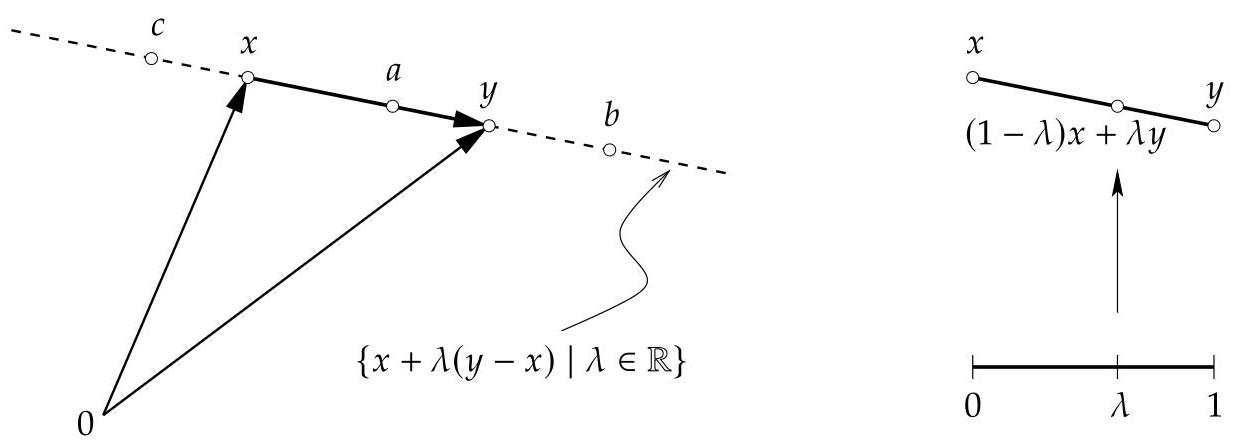
\includegraphics[width=0.8\linewidth]{images/ch05-fig06.jpg}
    \caption{左图:经过点 \(x\) 和 \(y\) 的直线由点 \(x + \lambda \left( {y - x}\right)\) 给出，其中 \(\lambda  \in  \mathbb{R}\) 。示例包括当 \(\lambda  = {0.6}\) 时的点 \(a\) 、当 \(\lambda  = {1.5}\) 时的点 \(b\) 以及当 \(\lambda  =  - {0.4}\) 时的点 \(c\) 。当 \(\lambda\) 限制在 \(0 \leq  \lambda  \leq  1\) 时得到连接 \(x\) 和 \(y\) 的线段。右图展示了实数区间 \(\left\lbrack  {0,1}\right\rbrack\) 如何通过映射 \(\lambda  \mapsto  \left( {1 - \lambda }\right) x + {\lambda y}\) 自然地映射到该线段上。}
  \end{figure}


例如，图5.5展示了定义在 \(u\left( x\right)  = \sqrt{x}\) 上的函数 \(\left\lbrack  {0,1}\right\rbrack\) 。在该函数的图(作为 \({\mathbb{R}}^{2}\) 的子集)上，我们展示了三个白色点，分别是点 \(\left( {x,u\left( x\right) }\right) ,\left( {\left( {1 - \lambda }\right) x + \lambda {x}^{\prime },u\left( {\left( {1 - \lambda }\right) x + \lambda {x}^{\prime }}\right) }\right)\) 和 \(\left( {{x}^{\prime },u\left( {x}^{\prime }\right) }\right)\) 。黑色点是外部白色点的凸组合 \(\left( {1 - \lambda }\right)  \cdot  \left( {x,u\left( x\right) }\right)  + \lambda  \cdot  \left( {{x}^{\prime },u\left( {x}^{\prime }\right) }\right)\) ，正如(5.46)中所断言的，它位于中间白色点的下方。这一情况普遍成立，表明 \(u\) 是凹函数。

如果(5.46)式取等号，那么函数图的那部分本身就是一条线段。如果永远不取等号，即只要 \(x \neq  {x}^{\prime }\) 和 \(0 < \lambda  < 1\) 时，(5.46)式以严格不等式成立，那么函数 \(u\) 被称为严格凹函数。

  \begin{figure}[H]\label{fig:5.5}
    \centering
    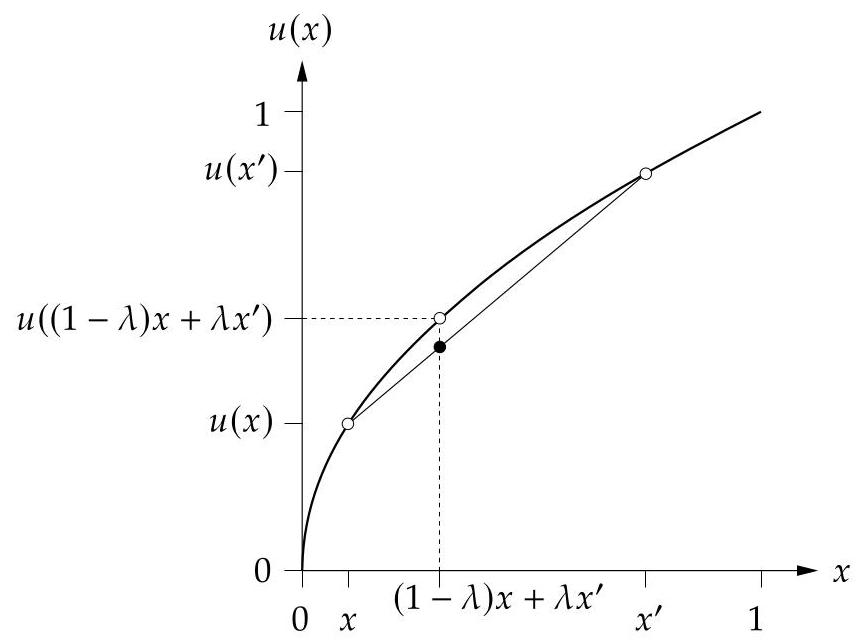
\includegraphics[width=0.8\linewidth]{images/ch05-fig07.jpg}
    \caption{区间 \(\left\lbrack  {0,1}\right\rbrack\) 上凹函数 \(u\left( x\right)  = \sqrt{x}\) 的示例。}
  \end{figure}


很容易看出，一个二次可微函数是凹函数，当且仅当它的二阶导数处处非正；如果它的二阶导数处处为负(例如 \(x > 0\) 时的平方根函数 \(\sqrt{x}\) )，则该函数是严格凹函数。此外，可以证明，除了函数定义域区间的端点外，凹性意味着连续性。

以下观察表明，风险厌恶等价于参与人的效用函数是凹函数。对于简单彩票，其证明几乎是直接的。

命题5.5。设 \(X\) 是一个实数区间， \(u : X \rightarrow  \mathbb{R}\) 是一个期望效用函数。考虑 \(X\) 上的任意彩票 \(P\) ，其期望值为 \(\widehat{x} = \mathbb{E}\left( P\right)\) 。那么参与人是风险厌恶的，即总是 \(P \precsim  \widehat{x}\) ，当且仅当 \(u\) 是凹函数。

证明。因为 \(X\) 是一个实数区间， \(X\) 上的任何彩票 \(P\) 都是一个具有期望值 \(\widehat{x} = \mathbb{E}\left( P\right)\) 的随机变量，其中 \(\widehat{x} \in  X\) 。首先考虑(见(5.16))一个简单彩票 \(P = x{ \land  }_{\lambda }{x}^{\prime }\) ，其中 \(\lambda  \in  \left\lbrack  {0,1}\right\rbrack\) 且 \(x,{x}^{\prime } \in  X\) ，这里 \(\widehat{x} = \mathbb{E}\left( P\right)  = \left( {1 - \lambda }\right) x + \lambda {x}^{\prime }\) 。那么 \(P \precsim  \widehat{x}\) 等价于 \(\mathbb{E}\left( {u,P}\right)  = \left( {1 - \lambda }\right) u\left( x\right)  + {\lambda u}\left( {x}^{\prime }\right)  \leq  u\left( \widehat{x}\right)\) ，这正是凹性条件(5.46)。

接下来需要证明，如果 \(u\) 是凹的，那么对于任何将正概率 \({p}_{1},\ldots ,{p}_{n}\) 分配给结果 \({x}_{1},\ldots ,{x}_{n}\) (其中 \(n \geq  3\) )的彩票 \(P\) ，有 \(P \precsim  \mathbb{E}\left( P\right)\) 。作为归纳假设，假设对于 \(n - 1\) 而非 \(n\) 这是成立的(我们刚刚已经证明了对于 \(n = 2\) 是成立的)。将 \(P\) 写为 \(Q{ \land  }_{{p}_{n}}{x}_{n}\) ，其中 \(Q\) 将概率 \(\frac{{p}_{i}}{1 - {p}_{n}}\) 分配给 \({x}_{i}\) (对于 \(1 \leq  i \leq  n - 1\) )。根据归纳假设， \(\mathbb{E}\left( {u,Q}\right)  \leq  u\left( {\mathbb{E}\left( Q\right) }\right)\) 。因此(其中第二个不等式成立是因为 \(u\) 是凹的)

\[
\mathbb{E}\left( {u,P}\right)  = \mathop{\sum }\limits_{{i = 1}}^{{n - 1}}{p}_{i}u\left( {x}_{i}\right)  + {p}_{n}u\left( {x}_{n}\right)
\]

\[
= \left( {1 - {p}_{n}}\right) \mathbb{E}\left( {u,Q}\right)  + {p}_{n}u\left( {x}_{n}\right)
\]

\[
\leq  \left( {1 - {p}_{n}}\right) u\left( {\mathbb{E}\left( Q\right) }\right)  + {p}_{n}u\left( {x}_{n}\right)
\]

\[
\leq  u\left( {\left( {1 - {p}_{n}}\right) \mathbb{E}\left( Q\right)  + {p}_{n}{x}_{n}}\right)  = u\left( {\mathbb{E}\left( P\right) }\right) ,
\]

这就完成了证明。

我们再次强调，风险厌恶要求结果是实值的，例如金钱，在这种情况下，彩票的期望本身就是一个可以与彩票进行比较的结果。

除了凹性之外，风险厌恶并不容易量化。如果参与人拥有 \(\widehat{x}\) 美元的财富并且是风险厌恶的，他会更喜欢确定的 \(\widehat{x}\) 美元，而不是在 \(\widehat{x} - {100}\) 美元和 \(\widehat{x} + {100}\) 美元之间进行等概率的赌博。因此，参与人应该愿意支付一个“风险溢价” \(\pi\) ，使得他对安全地获得 \(\widehat{x} - \pi\) 美元和进行赌博无差异。对于效用函数 \(u\left( x\right)  =  - {e}^{-{cx}}\) (对于某个 \(c > 0\) )，很容易看出 \(\pi\) 不依赖于 \(\widehat{x}\) ，并且在正仿射变换下，这是唯一具有此性质的凹效用函数。如果 \(\widehat{x}\) 的值是现实的，并且彩票本身(例如赢或输 100 美元)与所考虑的风险具有可比性，那么估计风险溢价 \(\pi\) 可能是构建效用函数的一种有用方法。

\section{延伸阅读}

蕴含期望效用函数存在的一致性公理有时被称为“理性公理”。当一个参与人按照自己一致的偏好行动时，他被称为“理性的”。在博弈论中，进一步的假设是所有参与人都了解整个博弈，包括所有参与人的偏好，每个人都是理性的，并且通常这是共同知识(每个人都知道每个人都知道，依此类推)。更详细的讨论请参见奥曼和布兰登伯格(1995 年)、奥曼和德雷兹(2008 年)以及佩雷亚(2012 年)的书。

博弈论以及一般的经济理论常常因这些理想化的假设而受到批评。应该明确的是，这些假设是数学模型的一部分，可能并不特别现实，在考虑博弈论分析的结论时需要对其进行质疑。当一个解(如均衡)不唯一时，这些结论就已经存在困难。但即使解是唯一的，这些结论也是规范的(陈述参与人应该做什么)而非描述性的(陈述参与人实际做了什么)。

对博弈论产生误解的另一个原因是，用于数学概念的词汇在其他地方有强烈的内涵。显然，博弈树并不是真正的树，而是描述了一系列决策“分支”，因此“树”可以作为一个中性的词汇。然而，“效用”这个词暗示了与结果的“有用性”相关的内在偏好强度。正如本章所论述的，它应该被视为一种用于表示对风险结果偏好的数学工具。

由于“效用”这个词的内涵，在本书的博弈背景下，我们改用更中性和积极的术语“收益”。然而，记住收益代表一种偏好，因此可以通过正仿射变换进行缩放是很有用的。

许多关于博弈论的经典著作，如卢斯和雷法(1957 年)以及迈尔森(1991 年)的著作，都始于证明使用期望效用合理性的理性假设。不同寻常的是，奥斯本和鲁宾斯坦(1994 年)甚至用偏好关系而非效用来定义博弈。

期望效用的概念通常归功于丹尼尔·伯努利(1738 年)，他提出用对数作为涉及货币的彩票的效用函数。关于这一概念的信息丰富且有趣的历史记载，可参见斯皮罗(2020 年)的著作，关于群体决策方法、孔多塞悖论和一般社会选择的内容也可参见斯皮罗(2010 年)的著作。期望效用函数的一致性公理由冯·诺依曼和摩根斯特恩(1947 年)提出，并且通常以他们的名字命名。图 5.2 中的悖论由阿莱(1953 年)描述。关于围绕这些公理的讨论的简短历史及更多参考文献，可参见莫斯卡蒂(2016 年)的著作。

一本关于效用理论的经典著作是菲什伯恩(1970 年)的作品，它将关于偏好的公理及其用效用函数表示的内容联系起来。赫斯坦和米尔诺(1953 年)提出的一种关于偏好的抽象方法被称为“混合集”，其中两个彩票(包括确定结果) \(P\) 和 \(Q\) 以及一个概率 \(\alpha\) 按照(5.15)式组合成一个新的彩票 \(\left( {1 - \alpha }\right) P + {\alpha Q}\) ，并且有关于这些 \(P,Q,\alpha\) 混合的合适公理。我们没有考虑这种抽象的“混合”，而是保留了它们作为彩票的含义，这样代数运算，例如在定理 5.4 的证明中使用的运算，就保持具体。

效用理论并不是一个很好的描述人类决策的理论，心理学家丹尼尔·卡尼曼和阿莫斯·特沃斯基对此进行了记录和广泛研究。刘易斯(2016 年)的科普书籍生动地描述了他们的合作与研究。非传递偏好的例子(5.10)由特沃斯基(1969 年)提出。

一篇关于风险厌恶的重要论文是普拉特(1964 年)的作品。

\section{ 第五章练习}

\begin{exercise}\label{exer:5.1}
在形式为 \(u\left( {{c}_{1},{c}_{2}}\right)  =\)  \({c}_{1} + w \cdot  {c}_{2}\) 的效用函数中找到正权重 \(w\) ，以使(5.10)中的候选人 \(x,y,z\) 之间至少有四种不同的严格排序。[提示:尝试一些 \(w\) 的值并改变它们。作为 \(w\) 的函数，三个候选人的 \(u\left( {{c}_{1},{c}_{2}}\right)\) 值是多少？]
\end{exercise}

\begin{exercise}\label{exer:5.2}
完成命题 5.2 中(5.21)式第三种情况 \({x}_{1} \prec  z\) 的证明，以表明 \(v\left( z\right)  = {au}\left( z\right)  + b\) 。如证明中所述，选择一个简单彩票 \(Q = {x}_{0}{ \land  }_{\gamma }z\) ，使得参与人对该彩票和 \({x}_{1}\) 无差异，然后使用(5.18)式和(5.20)式，按照(5.23)式的方式进行推导。
\end{exercise}

\begin{exercise}\label{exer:5.3}

(a) 对于满足 \(A < C\) 的实数 \(A,B,C\) ，证明等价关系(5.25)，包括其中的不等式。

(b) 证明两个彩票 \(P\) 和 \(R\) 的 \(\left( {1 - \alpha }\right) \mathbb{E}\left( {u,P}\right)  + \alpha \mathbb{E}\left( {u,R}\right)  = \mathbb{E}\left( {u,\left( {1 - \alpha }\right) P + {\alpha R}}\right)\) 关系，这是(5.30)式中的第二个等式。
\end{exercise}
